\documentclass[12pt, openany, oneside]{book}

\usepackage{listings}
\usepackage[dvipsnames]{xcolor}
\usepackage{ctex}
\usepackage{fontspec}
\usepackage{setspace}
\usepackage{tikz}
\usepackage{anyfontsize}
\usepackage{sectsty}
\usepackage{titlesec}
\usepackage{float}
\usepackage[hidelinks]{hyperref}
\usepackage[a4paper]{geometry}
\usepackage{url}
\usepackage{amssymb}
\usepackage{fontawesome5}
\usepackage[most]{tcolorbox}
\usepackage{stackengine}
\usepackage{multirow}
\usepackage{makecell}
\usepackage[T1]{fontenc}
\usepackage{diagbox}
\usepackage{longtable}
\usepackage{newtxtt}
\usepackage{pgf-umlcd}
\usepackage{bbding}
\usepackage{amsmath}
\usepackage{tkz-graph}
\usepackage{drawstack}
\usepackage{dcolumn}
\usepackage{tikzpeople}

\usetikzlibrary{calc,positioning,arrows,fit,shapes}
\usetikzlibrary{shapes.multipart,chains}
\usetikzlibrary{shadows}
\usetikzlibrary{arrows.meta}
\usetikzlibrary{matrix,backgrounds}

\tikzset{block/.style={
        font=\sffamily,
        draw=black,
        thin,
        fill=pink!50,
        rectangle split,
        rectangle split horizontal,
        rectangle split parts=#1,
        outer sep=0pt},
        gblock/.style={
            block,
            rectangle split parts=#1,
            fill=green!30}
        }

\makeatletter
\newcommand{\verbatimfont}[1]{\renewcommand{\verbatim@font}{\ttfamily#1}}
\makeatother

\makeatletter
\def\BState{\State\hskip-\ALG@thistlm}
\makeatother

\def\rlwd{.5pt} \def\rlht{2.2ex} \def\rldp{.5ex}
\def\mydiv#1{~
  \rule[-\rldp]{\rlwd}{\rlht}
  \setbox0=\hbox{~#1}
  \stackunder[\dimexpr\rldp-\rlwd]{~#1}{\rule{\wd0}{\rlwd}}
}

\definecolor{mycolor}{RGB}{0,128,128}
\newtcbox{\mybox} {
    on line,
    colback=mycolor,
    fontupper=\bfseries\color{white},
    boxrule=0pt,
    arc=5pt, 
    boxsep=0pt, 
    left=2pt, 
    right=2pt, 
    top=5pt, 
    bottom=5pt
}

\setstretch{1.5}
\setlength{\parindent}{0cm}

\geometry{a4paper,top=2.5cm,bottom=2.5cm}

\titleformat{\chapter}{\Huge\Huge\bfseries}{\chaptertitlename\ \thechapter{\ }}{0pt}{\Huge}{}
\titlespacing{\chapter}{0pt}{0pt}{12pt}

\definecolor{dkgreen}{rgb}{0,0.4,0}
\definecolor{gray}{rgb}{0.5,0.5,0.5}
\definecolor{mauve}{rgb}{0.58,0,0.82}
\definecolor{LightGray}{gray}{0.9}

\lstset{
    basicstyle=\linespread{1.3} \fontspec{Consolas},    %  the size of the fonts that are used for the code
	basewidth=0.5em,
    numbers=left,            % where to put the line-numbers
    numberstyle=\color{black},  % the style that is used for the line-numbers
    numbersep=10pt,                  % how far the line-numbers are from the code
    backgroundcolor=\color{white},
    showspaces=false,
    showstringspaces=false,
    showtabs=false,
    frame=single,                   % adds a frame around the code
    rulecolor=\color{black},        % if not set, the frame-color may be changed on line-breaks within not-black text (e.g. commens (green here))
    tabsize=4,                      % sets default tabsize to 2 spaces
    captionpos=t,                   % sets the caption-position to bottom
    breaklines=false,                % sets automatic line breaking
    breakatwhitespace=true,        % sets if automatic breaks should only happen at whitespace
    title=\lstname,                   % show the filename of files included with \lstinputlisting;
    % also try caption instead of title
    numberstyle=\color{black},		% line number color
    keywordstyle=\color{blue},          % keyword style
    commentstyle=\color{dkgreen},       % comment style
    stringstyle=\color{mauve},         % string literal style
    escapeinside={\%*}{*)},            % if you want to add LaTeX within your code
    morekeywords={*,...}               % if you want to add more keywords to the set
}

\begin{document}

\thispagestyle{empty}

\begin{tikzpicture}[overlay,remember picture]
	\fill[
		black!2]
	(current page.south west) rectangle (current page.north east);

	\shade[
		left color=Dandelion,
		right color=Dandelion!40,
		transform canvas ={rotate around ={45:($(current page.north west)+(0,-6)$)}}]
	($(current page.north west)+(0,-6)$) rectangle ++(9,1.5);

	\shade[
		left color=lightgray,
		right color=lightgray!50,
		rounded corners=0.75cm,
		transform canvas ={rotate around ={45:($(current page.north west)+(.5,-10)$)}}]
	($(current page.north west)+(0.5,-10)$) rectangle ++(15,1.5);

	\shade[
		left color=lightgray,
		rounded corners=0.3cm,
		transform canvas ={rotate around ={45:($(current page.north west)+(.5,-10)$)}}] ($(current page.north west)+(1.5,-9.55)$) rectangle ++(7,.6);

	\shade[
		left color=orange!80,
		right color=orange!60,
		rounded corners=0.4cm,
		transform canvas ={rotate around ={45:($(current page.north)+(-1.5,-3)$)}}]
	($(current page.north)+(-1.5,-3)$) rectangle ++(9,0.8);

	\shade[
		left color=red!80,
		right color=red!80,
		rounded corners=0.9cm,
		transform canvas ={rotate around ={45:($(current page.north)+(-3,-8)$)}}] ($(current page.north)+(-3,-8)$) rectangle ++(15,1.8);

	\shade[
		left color=orange,
		right color=Dandelion,
		rounded corners=0.9cm,
		transform canvas ={rotate around ={45:($(current page.north west)+(4,-15.5)$)}}]
	($(current page.north west)+(4,-15.5)$) rectangle ++(30,1.8);

	\shade[
		left color=RoyalBlue,
		right color=Emerald,
		rounded corners=0.75cm,
		transform canvas ={rotate around ={45:($(current page.north west)+(13,-10)$)}}]
	($(current page.north west)+(13,-10)$) rectangle ++(15,1.5);

	\shade[
		left color=lightgray,
		rounded corners=0.3cm,
		transform canvas ={rotate around ={45:($(current page.north west)+(18,-8)$)}}]
	($(current page.north west)+(18,-8)$) rectangle ++(15,0.6);

	\shade[
		left color=lightgray,
		rounded corners=0.4cm,
		transform canvas ={rotate around ={45:($(current page.north west)+(19,-5.65)$)}}]
	($(current page.north west)+(19,-5.65)$) rectangle ++(15,0.8);

	\shade[
		left color=OrangeRed,
		right color=red!80,
		rounded corners=0.6cm,
		transform canvas ={rotate around ={45:($(current page.north west)+(20,-9)$)}}]
	($(current page.north west)+(20,-9)$) rectangle ++(14,1.2);

	% Title
	\node[align=center] at ($(current page.center)+(0,-7)$)
	{
	{\fontsize{60}{60} \selectfont {{计算机网络}}}\\[1cm]
	{\fontsize{40}{40} \selectfont {{Computer Networking}}}\\[2cm]
	{\fontsize{20}{19.2} \selectfont \textcolor{orange}{ \bf 极夜酱}}\\[4pt]
	};
\end{tikzpicture}

\newpage

\pagestyle{plain}
\setcounter{page}{1}
\setcounter{tocdepth}{1}
\tableofcontents

\newpage

\setcounter{page}{1}

\chapter{网络}

\section{因特网}

\subsection{因特网(Internet)}

因特网是一个世界范围的计算机网络,它互联了遍及全世界数十亿的计算设备,所有这些设备都称为主机(host)或端系统(end system)。端系统通过通信链路(communication link)和分组交换机(packet switch)连接到一起,不同的链路能够以不同的速率传输数据,链路的传输速率(transmission rate)使用比特/秒(bps, bit/s)来度量。端系统通过因特网服务提供商(ISP, Internet Service Provider)接入因特网。\\

当一台端系统向另一台端系统发送数据时,发送端将数据分组,发送到目的端系统,在那里进行组装。一个分组所经历的一系列通信链路和分组交换机称为路径(route / path)。分组交换类似于现实中的货物运输,在出发地将货物分开并装上多辆卡车,每辆卡车独立通过公路运输,最后在目的地卸货并重新组装。\\

\subsection{分布式应用程序(Distributed Application)}

分布式应用程序涉及多个相互交换数据的端系统,例如即时通信、实时道路信息、视频会议、多人游戏等。分布式应用程序的核心问题在于一个端系统上的应用程序如何能够向运行在另一个端系统上的应用程序发送数据。\\

套接字接口(socket interface)规定了运行在一个端系统上的程序向运行在另一个端系统上的特定程序交付数据的方式。例如Alice要给Bob寄一封信,当然Alice不能只是写完这封信就把它丢出窗外。Alice需要把信放入信封,在信封上根据指定格式写上收信人的全名、地址和邮政编码,信封上贴上邮票,再将信封投入信箱中。Alice想要寄信就必须要遵守邮政服务制定的这一套规则。因此,发送数据的程序也必须遵守socket接口,才能向接收数据的程序发送数据。\\

\subsection{协议(Protocol)}

在两个人或两台设备之间进行通信时需要遵守一些协议,协议就是用于管理通信的一组规则。传输控制协议TCP(Transmission Control Protocol)和网际协议IP(Internet Protocol)是因特网中两个最为重要的协议,因特网的主要协议统称为TCP/IP。\\

因特网标准(Internet standard)是经过充分测试的规约,只要是与因特网打交道,就会用到它们,并要服从于它们。因特网标准由IETF(Internet Engineering Task Force)研发,IETF的标准文档称为RFC (Request For Comment),目的是解决因特网先驱者们面临的网络和协议问题。它们定义了TCP、IP、HTTP、SMTP等协议,目前已经有将近7000个RFC。\\

人类无时无刻都在执行协议,人类用约定好的交互方式互相交流。但是如果两人的交谈都不在同一频道上,那就不能好好沟通了。\\

\begin{figure}[H]
    \centering
    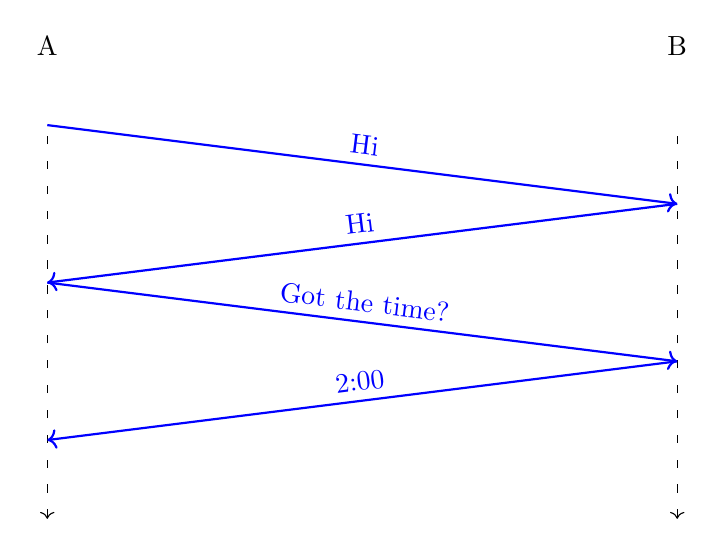
\begin{tikzpicture}
        \node at (0,6) {A};
        \node at (8,6) {B};

        \draw[loosely dashed, <-] (0,0) -- (0,5);
        \draw[loosely dashed, <-] (8,0) -- (8,5);

        \draw[blue, ->, thick] (0,5) -- (8,4) node[above, midway, sloped]{Hi};
        \draw[blue, ->, thick] (8,4) -- (0,3) node[above, midway, sloped]{Hi};
        \draw[blue, ->, thick] (0,3) -- (8,2) node[above, midway, sloped]{Got the time?};
        \draw[blue, ->, thick] (8,2) -- (0,1) node[above, midway, sloped]{2:00};
    \end{tikzpicture}
    \caption{人类协议}
\end{figure}

在因特网中,涉及两个或多个远程通信实体的所有活动都受协议的制约。例如在浏览器中输入URL(Uniform Resource Locator)向一个Web服务器发出请求,首先你的计算机将向该Web服务器发送一条连接请求报文,并等待回答。Web服务器接收到连接请求报文,并返回一条连接响应报文。在得知请求正常后,计算机会发送一条要获取的网页名字的报文,最后Web服务器向计算机返回该网页。\\

\begin{figure}[H]
    \centering
    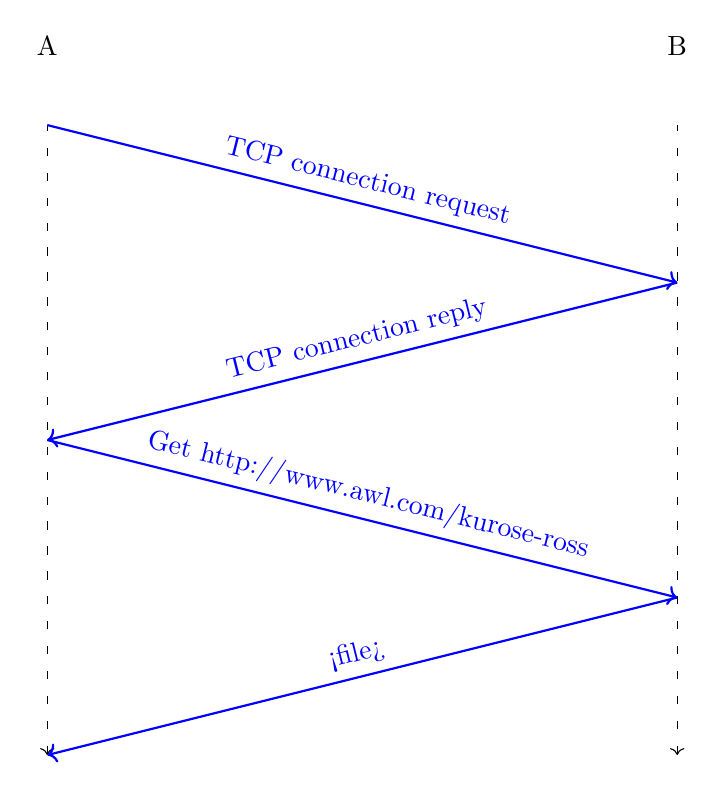
\begin{tikzpicture}
        \node at (0,9) {A};
        \node at (8,9) {B};

        \draw[loosely dashed, <-] (0,0) -- (0,8);
        \draw[loosely dashed, <-] (8,0) -- (8,8);

        \draw[blue, ->, thick] (0,8) -- (8,6) node[above, midway, sloped]{TCP connection request};
        \draw[blue, ->, thick] (8,6) -- (0,4) node[above, midway, sloped]{TCP connection reply};
        \draw[blue, ->, thick] (0,4) -- (8,2) node[above, midway, sloped]{Get http://www.awl.com/kurose-ross};
        \draw[blue, ->, thick] (8,2) -- (0,0) node[above, midway, sloped]{<file>};
    \end{tikzpicture}
    \caption{网络协议}
\end{figure}

\newpage

\section{分组交换}

\subsection{存储转发传输(Store-and-Forward Transmission)}

在网络应用中,端系统彼此交换报文(message),报文能够包含任何数据。报文从源端系统发送到目的端系统的过程中,长报文会被划分为较小的数据块,称为分组(packet),每个分组都通过通信链路和分组交换机传送。如果源端系统发送一个$ L $ bits分组,链路的传输速率为$ R $ bits/sec,则传输该分组的时间为$ L \over R $秒。\\

多数分组交换机在链路的输入端使用存储转发传输机制,存储转发传输是指在交换机能够开始向输出链路传输该分组的第一个bit之前,必须接收到整个分组。\\

\begin{figure}[H]
    \centering
    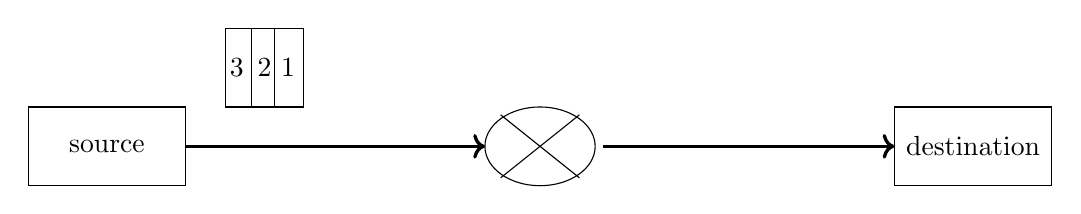
\begin{tikzpicture}
        \draw (0,0) rectangle (2,1);
        \node at (1,0.5) {source};
        \draw (11,0) rectangle (13,1);
        \node at (12,0.5) {destination};
        \draw (6.5,0.5) ellipse (0.7 and 0.5);
        \draw[-] (6,0.9) -- (7,0.1);
        \draw[-] (7,0.9) -- (6,0.1);

        \draw[->, very thick] (2,0.5) -- (5.8,0.5);
        \draw[->, very thick] (7.3,0.5) -- (11,0.5);

        \draw (2.5,1) rectangle (3.5,2);
        \draw (2.833,1) -- (2.833,2);
        \draw (3.133,1) -- (3.133,2);
        \node at (2.65,1.5) {3};
        \node at (3,1.5) {2};
        \node at (3.3,1.5) {1};
    \end{tikzpicture}
    \caption{存储转发}
\end{figure}

假设忽略传播时延(propagation delay),源端系统在时间0开始传输,路由器在时间$ L \over R $刚好接收到整个分组,之后再向输出链路开始传输,在时间$ 2 {L \over R} $整个分组被目的端系统接收。\\

因此,由$ N $条速率为$ R $的链路组成的路径(在源和目的地之间有$ N - 1 $台路由器)发送一个分组,端到端的时延为

\vspace{-0.5cm}

\begin{align}
    d = N {L \over R}
\end{align}

\vspace{0.5cm}

\subsection{时延}

当从一个节点到后继节点,一个分组在沿途的每个节点都经受了几种不同类型的时延,包括节点处理时延(nodal processing delay)、排队时延(queuing delay)、传输时延(transmission delay)、传播时延(propagation delay)。\\

处理时延包括了检查分组首部和决定分组去向所需要的时间,以及检查差错的时间。\\

分组交换机的每条链路都有一个输出缓存/输出队列(output buffer / output queue)。如果到达的分组需要传输到某条链路,但发现该链路正忙于传输其它分组,该分组必须在输出缓存中等待。因此,除了存储转发时延以外,分组还要承受输出缓存的排队时延。由于缓存空间的大小是有限的,到达的分组可能发现该缓存已被填满,这种情况下将出现丢包(packet loss),到达的分组或已经排队的分组将被丢弃。\\

\begin{figure}[H]
    \centering
    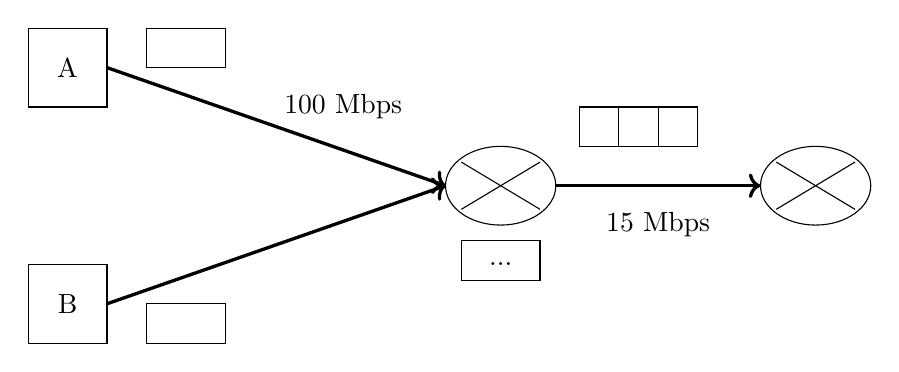
\begin{tikzpicture}
        \draw (0,1) rectangle (1,2);
        \node at (0.5,1.5) {A};
        \draw (0,-2) rectangle (1,-1);
        \node at (0.5,-1.5) {B};

        \draw (6,0) ellipse (0.7 and 0.5);
        \draw[-] (5.5,0.3) -- (6.5,-0.3);
        \draw[-] (5.5,-0.3) -- (6.5,0.3);

        \draw[->, very thick] (1,1.5) -- (5.3,0);
        \draw[->, very thick] (1,-1.5) -- (5.3,0);

        \draw (1.5,1.5) rectangle (2.5,2);
        \draw (1.5,-2) rectangle (2.5,-1.5);
        \node at (4,1) {100 Mbps};

        \draw (10,0) ellipse (0.7 and 0.5);
        \draw[-] (9.5,0.3) -- (10.5,-0.3);
        \draw[-] (9.5,-0.3) -- (10.5,0.3);

        \draw[->, very thick] (6.7,0) -- (9.3,0);

        \draw (7,0.5) rectangle (8.5,1);
        \draw[-] (7.5,0.5) -- (7.5,1);
        \draw[-] (8,0.5) -- (8,1);
        \node at (8,-0.5) {15 Mbps};

        \draw (5.5,-1.2) rectangle (6.5,-0.7);
        \node at (6,-1) {...};
    \end{tikzpicture}
    \caption{排队时延}
\end{figure}

分组通常是以FCFS(First-Come-First-Served)的方式传输,只有当所有已经到达的分组被传输之后,才能传输新到达的分组。传输时延$ L \over R $就是将所有分组推向输出链路所需的时间。\\

传播时延是指从链路的起点到下一个路由器传播所需的时间。\\

假设$ d_{proc} $、$ d_{queue} $、$ d_{trans} $和$ d_{prop} $分别表示处理时延、排队时延、传输时延和传播时延,那么节点总时延为

\vspace{-0.5cm}

\begin{align}
    d_{nodal} = d_{proc} + d_{queue} + d_{trans} + d_{prop}
\end{align}

\begin{figure}[H]
    \centering
    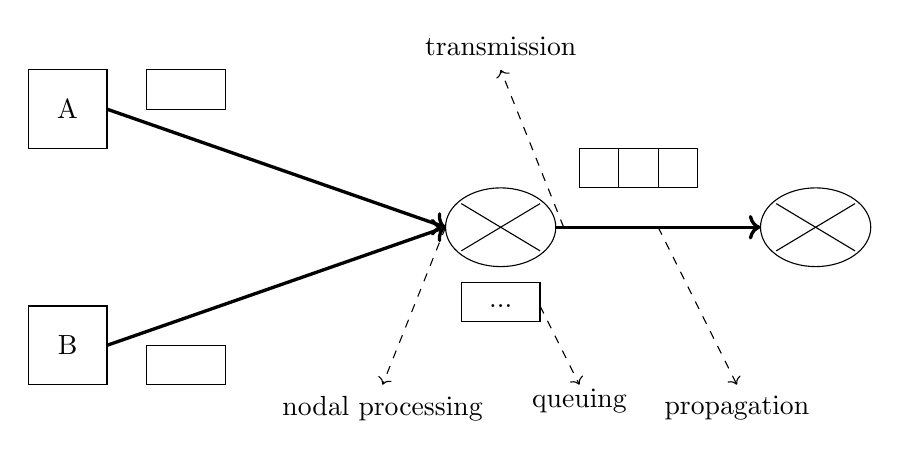
\begin{tikzpicture}
        \draw (0,1) rectangle (1,2);
        \node at (0.5,1.5) {A};
        \draw (0,-2) rectangle (1,-1);
        \node at (0.5,-1.5) {B};

        \draw (6,0) ellipse (0.7 and 0.5);
        \draw[-] (5.5,0.3) -- (6.5,-0.3);
        \draw[-] (5.5,-0.3) -- (6.5,0.3);

        \draw[->, very thick] (1,1.5) -- (5.3,0);
        \draw[->, very thick] (1,-1.5) -- (5.3,0);

        \draw (1.5,1.5) rectangle (2.5,2);
        \draw (1.5,-2) rectangle (2.5,-1.5);

        \draw (10,0) ellipse (0.7 and 0.5);
        \draw[-] (9.5,0.3) -- (10.5,-0.3);
        \draw[-] (9.5,-0.3) -- (10.5,0.3);

        \draw[->, very thick] (6.7,0) -- (9.3,0);

        \draw (7,0.5) rectangle (8.5,1);
        \draw[-] (7.5,0.5) -- (7.5,1);
        \draw[-] (8,0.5) -- (8,1);

        \draw (5.5,-1.2) rectangle (6.5,-0.7);
        \node at (6,-1) {...};
        \draw[dashed, ->] (6.5,-1) -- (7,-2);
        \node at (7,-2.2) {queuing};

        \draw[dashed, ->] (5.3,0) -- (4.5,-2);
        \node at (4.5,-2.3) {nodal processing};

        \draw[dashed, ->] (6.8,0) -- (6,2);
        \node at (6,2.3) {transmission};

        \draw[dashed, ->] (8,0) -- (9,-2);
        \node at (9,-2.3) {propagation};
    \end{tikzpicture}
    \caption{时延}
\end{figure}

\vspace{0.5cm}

\subsection{转发表(Forwarding Table)}

路由器从输入链路获得分组,然后向输出链路发送分组,但是路由器怎样决定应当向哪一条链路发送呢?\\

因特网中每一个端系统都有一个IP地址,源在发送分组时在分组首部包含了目的地的IP地址。当分组到达每一个路由器时,路由器根据转发表,为其查询适当的输出链路。\\

端到端的选路过程类似于现实中的问路,每到一个地点都询问别人路线,逐步找到最终的目的地。在这个类比中,被问路的人就类似于路由器。\\

\subsection{traceroute}

traceroute是诊断网络问题时常用的工具,它可以定位从源主机到目标主机之间经过了哪些路由器,以及到达各个路由器的耗时。当源主机向目标主机发送消息,发现消息无法送达。此时,可能是某个中间节点发生了问题,比如某个路由器因负载过高产生了丢包。通过traceroute可以定位网络包在是在哪个节点丢失的。\\

traceroute将从源发送N个特殊的分组,当第i个路由器收到第i个分组时,该路由器会向源回送一个报文,记录了路由器的名字和地址。traceroute会重复该实验3次。\\

\mybox{traceroute (Linux) / tracert (Windows)}

\begin{lstlisting}
tracert www.github.com
\end{lstlisting}

\begin{tcolorbox}
    \mybox{运行结果}
    \begin{verbatim}
1     2 ms     9 ms     2 ms  HS8145V [192.168.1.1]
2     5 ms    15 ms     5 ms  100.65.0.1
3     5 ms     5 ms     5 ms  124.74.22.41
4    25 ms     6 ms    17 ms  101.95.88.138
5     *        *        *     请求超时。
6     *        *        *     请求超时。
7     *        *        *     请求超时。
8    30 ms    32 ms    35 ms  106.38.244.146
9     *        *        *     请求超时。
10     *        *        *     请求超时。
11     *        *        *     请求超时。
12    30 ms    31 ms    31 ms  220.181.38.251
	\end{verbatim}
\end{tcolorbox}

\newpage

\section{协议层}

\subsection{协议栈(protocol stack)}

因特网是个极其复杂的系统,因此因特网的体系存在分层的组织结构。类似一次乘飞机的过程,首先需要购票、托运行李、登机,飞行到目的地后,需要离机、认领行李,如果对航班不满意,还可以在向票务机构投诉。\\

\begin{figure}[H]
    \centering
    \begin{tikzpicture}
        \draw (-7,8) rectangle (-3,9);
        \node at (-5,8.5) {票务(购票)};

        \draw (-7,6) rectangle (-3,7);
        \node at (-5,6.5) {行李(托运)};

        \draw (-7,4) rectangle (-3,5);
        \node at (-5,4.5) {登机口(登机)};

        \draw (-7,2) rectangle (-3,3);
        \node at (-5,2.5) {跑道(起飞)};

        \draw (-2,0) rectangle (2,1);
        \node at (0,0.5) {飞行};

        \draw (7,2) rectangle (3,3);
        \node at (5,2.5) {跑道(降落)};

        \draw (7,4) rectangle (3,5);
        \node at (5,4.5) {登机口(离机)};

        \draw (7,6) rectangle (3,7);
        \node at (5,6.5) {行李(认领)};

        \draw (7,8) rectangle (3,9);
        \node at (5,8.5) {票务(投诉)};

        \draw[->] (-5,8) -- (-5,7);
        \draw[->] (-5,6) -- (-5,5);
        \draw[->] (-5,4) -- (-5,3);
        \draw[->] (-5,2) -- (-2,1);
        \draw[->] (2,1) -- (5,2);
        \draw[->] (5,3) -- (5,4);
        \draw[->] (5,5) -- (5,6);
        \draw[->] (5,7) -- (5,8);
    \end{tikzpicture}
    \caption{航行流程}
\end{figure}

协议分层是为了使各层之间相互独立,每一层只专注于做一类事情。各层之间相互独立,各层之间不需要关心其它层是如何实现的,只需要知道自己如何调用下层提供好的功能就可以。同时协议分层提高了整体灵活性,每一层都可以使用最适合的技术来实现,只需要保证提供的功能以及暴露的接口的规则没有改变就行。\\

各层的所有协议被称为协议栈,TCP/IP协议栈由5个层次组成,分为是物理层、链路层、网络层、传输层和应用层。\\

ISO(International Organization for Standard)为了更好地使网络应用更为普及,推出了OSI(Open System Interconnection)参考模型。但因为OSI七层模型出现地比TCP/IP五层模型晚,在OSI开始使用之前,TCP/IP已经被广泛使用,最终OSI没有在实践中被广泛应用。\\

\begin{table}[H]
    \centering
    \setlength{\tabcolsep}{5mm}{
        \begin{tabular}{|c|l|}
            \hline
            \textbf{协议层} & \textbf{功能}                         \\
            \hline
            应用层          & 提供网络服务操作接口                  \\
            \hline
            表示层          & 对要传输的数据进行处理                \\
            \hline
            会话层          & 管理不同通讯节点之间的连接信息        \\
            \hline
            传输层          & 建立不同节点之间的网络连接            \\
            \hline
            网络层          & 将网络地址映射为MAC地址实现数据包转发 \\
            \hline
            数据链路层      & 将要发送的数据包转为数据帧            \\
            \hline
            物理层          & 利用物理设备实现数据的传输            \\
            \hline
        \end{tabular}
    }
    \caption{OSI七层模型}
\end{table}

\vspace{0.5cm}

\begin{figure}[H]
    \centering
    \begin{tikzpicture}
        \draw (0,0) rectangle (3,7);
        \draw (8,0) rectangle (11,7);
        \draw (0,1) -- (3,1);
        \draw (0,2) -- (3,2);
        \draw (0,3) -- (3,3);
        \draw (0,4) -- (3,4);
        \draw (0,5) -- (3,5);
        \draw (0,6) -- (3,6);
        \draw (8,1) -- (11,1);
        \draw (8,2) -- (11,2);
        \draw (8,3) -- (11,3);
        \draw (8,4) -- (11,4);
        \draw (8,5) -- (11,5);
        \draw (8,6) -- (11,6);

        \draw (1.5,6.5) node{应用层};
        \draw (1.5,5.5) node{表示层};
        \draw (1.5,4.5) node{会话层};
        \draw (1.5,3.5) node{传输层};
        \draw (1.5,2.5) node{网络层};
        \draw (1.5,1.5) node{数据链路层};
        \draw (1.5,0.5) node{物理层};
        \draw (9.5,6.5) node{应用层};
        \draw (9.5,5.5) node{表示层};
        \draw (9.5,4.5) node{会话层};
        \draw (9.5,3.5) node{传输层};
        \draw (9.5,2.5) node{网络层};
        \draw (9.5,1.5) node{数据链路层};
        \draw (9.5,0.5) node{物理层};

        \draw[->, very thick] (-1,7) -- (-1,0);
        \draw[->, very thick] (12,0) -- (12,7);
        \draw[->] (1.5,0) -- (1.5,-1) -- (9.5,-1) -- (9.5,0);
    \end{tikzpicture}
    \caption{数据传输}
\end{figure}

\vspace{0.5cm}

\subsection{封装(Encapsulation)}

在发送主机端,应用层报文(application-layer message)被传送给传输层,传输层收取到报文并附加首部信息,形成传输层报文段(transport-layer segment),被添加的首部将被接收端的传输层使用。首部信息包括了交付应用程序信息、差错检测位信息等。\\

传输层继续向网络层传递该报文段,网络层再添加首部信息,如源和目的端系统地址等,形成了网络层数据报(network-layer datagram)。\\

该数据报接下来被传递给链路层,链路层添加其首部信息,形成链路层帧(link-layer frame)。\\

\begin{figure}[H]
    \centering
    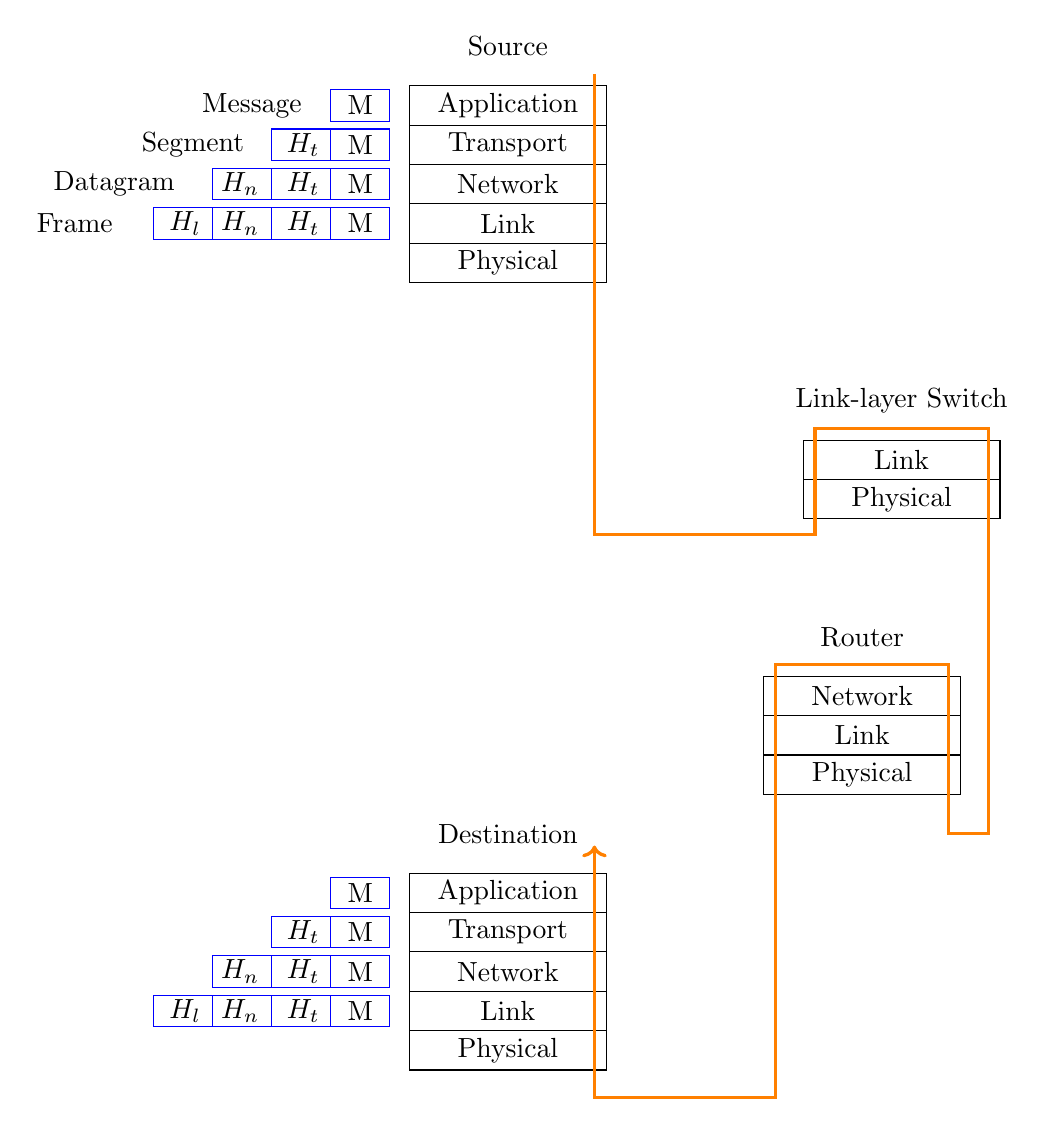
\begin{tikzpicture}
        \draw (0,0) rectangle (2.5,2.5);
        \draw (0,0.5) -- (2.5,0.5);
        \draw (0,1) -- (2.5,1);
        \draw (0,1.5) -- (2.5,1.5);
        \draw (0,2) -- (2.5,2);
        \draw (0,2.5) -- (2.5,2.5);
        \draw (1.25,2.25) node {Application};
        \draw (1.25,1.75) node {Transport};
        \draw (1.25,1.25) node {Network};
        \draw (1.25,0.75) node {Link};
        \draw (1.25,0.25) node {Physical};
        \draw (1.25,3) node {Source};

        \draw[blue] (-1,2.05) rectangle (-0.25,2.45);
        \draw (-0.625,2.25) node {M};
        \draw (-2,2.25) node {Message};
        \draw[blue] (-1.75,1.55) rectangle (-0.25,1.95);
        \draw[blue] (-1,1.55) -- (-1,1.95);
        \draw (-0.625,1.75) node {M};
        \draw (-1.35,1.75) node {$ H_t $};
        \draw (-2.75,1.75) node {Segment};
        \draw[blue] (-2.5,1.05) rectangle (-0.25,1.45);
        \draw[blue] (-1,1.05) -- (-1,1.45);
        \draw[blue] (-1.75,1.05) -- (-1.75,1.45);
        \draw (-0.625,1.25) node {M};
        \draw (-1.35,1.25) node {$ H_t $};
        \draw (-2.15,1.25) node {$ H_n $};
        \draw (-3.75,1.25) node {Datagram};
        \draw[blue] (-3.25,0.55) rectangle (-0.25,0.95);
        \draw[blue] (-1,0.55) -- (-1,0.95);
        \draw[blue] (-1.75,0.55) -- (-1.75,0.95);
        \draw[blue] (-2.5,0.55) -- (-2.5,0.95);
        \draw (-0.625,0.75) node {M};
        \draw (-1.35,0.75) node {$ H_t $};
        \draw (-2.15,0.75) node {$ H_n $};
        \draw (-2.85,0.75) node {$ H_l $};
        \draw (-4.25,0.75) node {Frame};

        \draw (0,-10) rectangle (2.5,-7.5);
        \draw (0,-9.5) -- (2.5,-9.5);
        \draw (0,-9) -- (2.5,-9);
        \draw (0,-8.5) -- (2.5,-8.5);
        \draw (0,-8) -- (2.5,-8);
        \draw (0,-7.5) -- (2.5,-7.5);
        \draw (1.25,-7.75) node {Application};
        \draw (1.25,-8.25) node {Transport};
        \draw (1.25,-8.75) node {Network};
        \draw (1.25,-9.25) node {Link};
        \draw (1.25,-9.75) node {Physical};
        \draw (1.25,-7) node {Destination};

        \draw[blue] (-1,-7.95) rectangle (-0.25,-7.55);
        \draw (-0.625,-7.75) node {M};
        \draw[blue] (-1.75,-8.45) rectangle (-0.25,-8.05);
        \draw[blue] (-1,-8.45) -- (-1,-8.05);
        \draw (-0.625,-8.25) node {M};
        \draw (-1.35,-8.25) node {$ H_t $};
        \draw[blue] (-2.5,-8.95) rectangle (-0.25,-8.55);
        \draw[blue] (-1,-8.95) -- (-1,-8.55);
        \draw[blue] (-1.75,-8.95) -- (-1.75,-8.55);
        \draw (-0.625,-8.75) node {M};
        \draw (-1.35,-8.75) node {$ H_t $};
        \draw (-2.15,-8.75) node {$ H_n $};
        \draw[blue] (-3.25,-9.45) rectangle (-0.25,-9.05);
        \draw[blue] (-1,-9.45) -- (-1,-9.05);
        \draw[blue] (-1.75,-9.45) -- (-1.75,-9.05);
        \draw[blue] (-2.5,-9.45) -- (-2.5,-9.05);
        \draw (-0.625,-9.25) node {M};
        \draw (-1.35,-9.25) node {$ H_t $};
        \draw (-2.15,-9.25) node {$ H_n $};
        \draw (-2.85,-9.25) node {$ H_l $};

        \draw (5,-2) rectangle (7.5,-3);
        \draw (5,-2.5) -- (7.5,-2.5);
        \draw (6.25,-2.25) node {Link};
        \draw (6.25,-2.75) node {Physical};
        \draw (6.25,-1.5) node {Link-layer Switch};

        \draw (4.5,-5) rectangle (7,-6.5);
        \draw (4.5,-5.5) -- (7,-5.5);
        \draw (4.5,-6) -- (7,-6);
        \draw (5.75,-5.25) node {Network};
        \draw (5.75,-5.75) node {Link};
        \draw (5.75,-6.25) node {Physical};
        \draw (5.75,-4.5) node {Router};

        \draw[->, very thick, orange] (2.35,2.65) -- (2.35,-3.2) -- (5.15,-3.2) -- (5.15,-1.85) -- (7.35,-1.85) -- (7.35,-7) -- (6.85,-7) -- (6.85,-4.85) -- (4.65,-4.85) -- (4.65,-10.35) -- (2.35,-10.35) -- (2.35,-7.15);
    \end{tikzpicture}
    \caption{封装}
\end{figure}

\newpage

\section{网络安全}

\subsection{网络攻击}

2000年2月7日,化名MafiaBoy的15岁加拿大少年攻击了Yahoo、Amazon和eBay,使这些网站瘫痪达数小时,造成了超过12亿美元的损失,在股市中造成混乱。MafiaBoy后来被透露为一名名叫Michael Calce的高中生,通过入侵几所大学的网络并利用其服务器进行DDoS攻击。这次袭击直接导致了今天许多网络犯罪法的制定。现在MafiaBoy已经金盆洗手,从事网络安全行业工作。\\

2017年1月,University of Albert内20个教室和实验室的300台电脑被安装恶意软件,导致近3000名学生的用户信息被盗。\\

2017年4月,一名Laurentian University的CS学生为了证明学校的系统容易受到攻击,从而入侵了学校系统,导致近2000名学生的个人记录(包括密码、电话号码、成绩等)被泄漏。\\

因特网最初的设计理念是让一群相互信任的用户连接到一个透明的网络上,因此安全性并没有太过必要。然而如今的网络不再是完全透明和相互信任的,因此网络安全领域需要研究如何攻击计算机网络、如何防御免受攻击和如何设计能够更好地避免攻击的体系。\\

\subsection{恶意软件}

多数的恶意软件(malware)通过自我复制(self-replicating)传播,一旦设备感染了恶意软件,就有可能导致文件丢失、隐私泄漏等。恶意软件能够以病毒(virus)或蠕虫(worm)的形式传播。病毒是利用用户交互来感染用户设备的,例如包含恶意代码的电子邮件附件,如果用户无意打开附件,就会在其设备上运行恶意软件。另一种蠕虫则无需任何用户交互,例如用户在使用某些比较脆弱的网络应用程序时,该应用可能用因特网接受恶意软件并运行。\\

\subsection{DoS攻击}

另一种通过攻击服务器和网络基础设施的威胁称为拒绝服务攻击(DoS, Denial-of-Service)。例如泛洪攻击,攻击者通过向目标主机发送大量的分组,堵塞目标的接入链路,使得合法分组无法到达服务器。但是如果服务器的接入速率非常大的话,单一的攻击源无法产生足够大的流量来伤害服务器。因此攻击者可以通过控制多个源向目标发送大量流量,这种方法称为分布式DoS(DDoS, Distributed DoS)。\\

\begin{figure}[H]
    \centering
    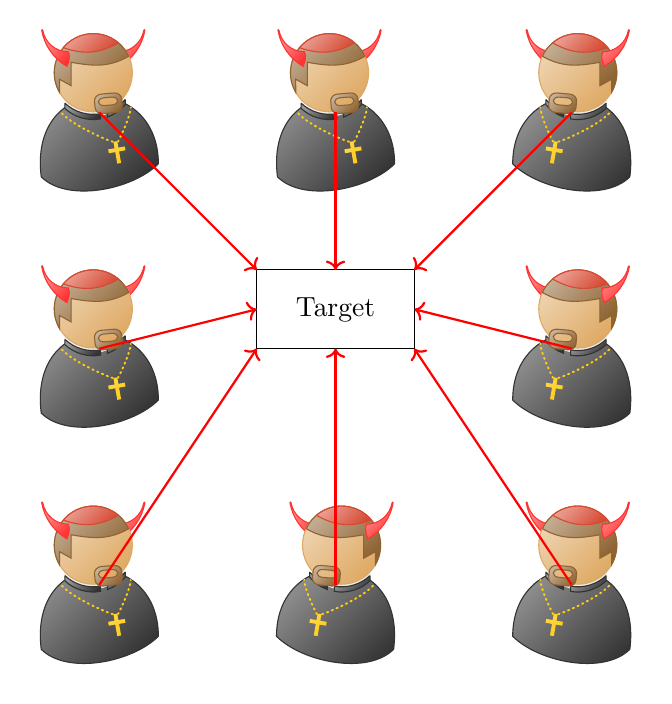
\begin{tikzpicture}[every node/.style={minimum width=1.5cm}]
        \draw (0,0) rectangle (2,1);
        \node at (1,0.5) {Target};

        \node[priest, evil] at (-2,3) {};
        \node[priest, evil] at (-2,0) {};
        \node[priest, evil] at (-2,-3) {};
        \node[priest, evil] at (1,3) {};
        \node[priest, evil, mirrored] at (4,3) {};
        \node[priest, evil, mirrored] at (4,0) {};
        \node[priest, evil, mirrored] at (4,-3) {};
        \node[priest, evil, mirrored] at (1,-3) {};

        \draw[->, thick, red] (-2,3) -- (0,1);
        \draw[->, thick, red] (-2,0) -- (0,0.5);
        \draw[->, thick, red] (-2,-3) -- (0,0);
        \draw[->, thick, red] (1,3) -- (1,1);
        \draw[->, thick, red] (4,3) -- (2,1);
        \draw[->, thick, red] (4,0) -- (2,0.5);
        \draw[->, thick, red] (4,-3) -- (2,0);
        \draw[->, thick, red] (1,-3) -- (1,0);
    \end{tikzpicture}
    \caption{DDoS}
\end{figure}

\vspace{0.5cm}

\subsection{IP欺骗(IP Spoofing)}

IP欺骗是指伪造源IP地址,以便冒充其它系统或发件人的身份,从而冒充另外一台机器与服务器打交道。IP欺骗会造成目标系统受到攻击却无法确认攻击源,或者取得目标系统的信任以便获取机密信息。IP欺骗的防范,一方面需要目标设备采取更强有力的认证措施,不仅仅根据源IP就信任来访者,还需要更多的认证手段。\\

\begin{figure}[H]
    \centering
    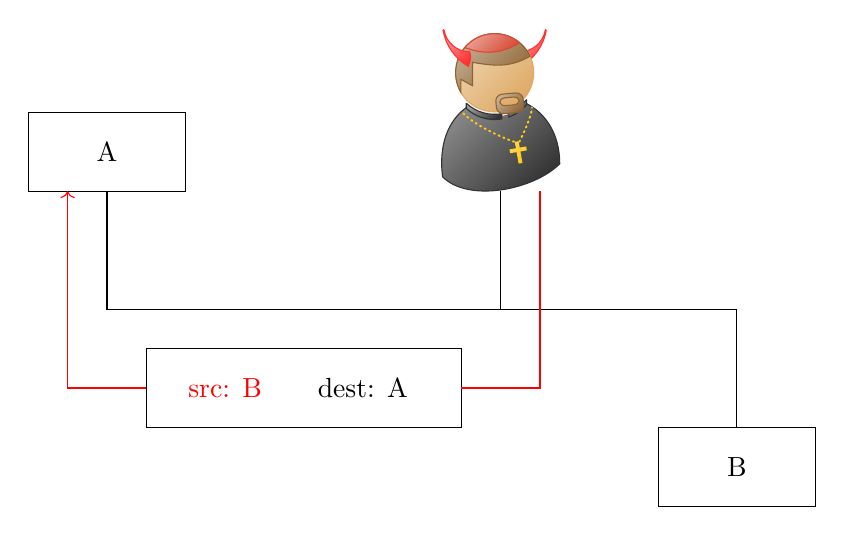
\begin{tikzpicture}[every node/.style={minimum width=1.5cm}]
        \draw (0,0) rectangle (2,1);
        \node at (1,0.5) {A};

        \draw (8,-4) rectangle (10,-3);
        \node at (9,-3.5) {B};

        \node[priest, evil] at (6,1) {};

        \draw (1,0) -- (1,-1.5) -- (9,-1.5) -- (9,-3);
        \draw (6,0) -- (6,-1.5);

        \draw (1.5,-3) rectangle (5.5,-2);
        \node[red] at (2.5,-2.5) {src: B};
        \node at (4.25,-2.5) {dest: A};

        \draw[red] (6.5,0) -- (6.5,-2.5) -- (5.5,-2.5);
        \draw[red, ->] (1.5,-2.5) -- (0.5,-2.5) -- (0.5,0);
    \end{tikzpicture}
    \caption{IP欺骗}
\end{figure}

\newpage
\chapter{应用层}

\section{应用层协议}

\subsection{网络应用}

网络应用程序是指能够运行在不同端系统并通过网络彼此通信的程序。例如在Web应用程序中,有两个互相通信的程序,一个是运行在用户主机上的浏览器程序,另一个是运行在Web服务器主机上的服务器程序。\\

应用程序体系结构包括Client-Server和P2P(Peer-to-Peer)两种体系结构。在Client-Server中,服务器主机一直运行处理客户端的请求。因为服务器需要有一个固定的的IP地址,因此客户端能够通过IP地址发送分组与其联系。著名的Client-Server应用程序包括Web、FTP、Telnet和电子邮件等。在Client-Server应用中,经常会出现一台单独的服务器主机不堪重负,跟不上所有客户请求的情况。例如搜索引擎(如Google、Bing、Baidu)、电商(如Amazon、eBay、Alibaba)、电子邮件(如Gmail、Yahoo!)、社交媒体(如Facebook、Instagram、Twitter、WeChat)都分步了多个数据中心,每数据中心都有数十万台服务器,必须要持续供电和维护。而在P2P中,主机之间的通信不必通过专门的服务器,很多流量密集型的应用都是P2P体系结构的,包括对等方协助下载加速器(如迅雷)、文件共享(如BitTorrent)。\\

\subsection{进程通信}

在同一个端系统中,多个进程可以通过进程间通信的机制相互通信,然而在不同的端系统(可能有不同的操作系统)中,需要通过网络交换报文(message)。进程通过套接字(socket)接口向网络发送或接收报文。\\

\begin{figure}[H]
    \centering
    \begin{tikzpicture}
        \draw (0,0) rectangle (3,9);
        \draw (8,0) rectangle (11,9);
        \draw (0,1) -- (3,1);
        \draw (0,2) -- (3,2);
        \draw (0,3) -- (3,3);
        \draw (0,4) -- (3,4);
        \draw (0,5) -- (3,5);
        \draw (0,6.5) -- (3,6.5);
        \draw (8,1) -- (11,1);
        \draw (8,2) -- (11,2);
        \draw (8,3) -- (11,3);
        \draw (8,4) -- (11,4);
        \draw (8,5) -- (11,5);
        \draw (8,6.5) -- (11,6.5);

        \draw (1.5,8.5) node{应用层};
        \draw (1.5,5.5) node{表示层};
        \draw (1.5,4.5) node{会话层};
        \draw (1.5,3.5) node{传输层};
        \draw (1.5,2.5) node{网络层};
        \draw (1.5,1.5) node{数据链路层};
        \draw (1.5,0.5) node{物理层};
        \draw (9.5,8.5) node{应用层};
        \draw (9.5,5.5) node{表示层};
        \draw (9.5,4.5) node{会话层};
        \draw (9.5,3.5) node{传输层};
        \draw (9.5,2.5) node{网络层};
        \draw (9.5,1.5) node{数据链路层};
        \draw (9.5,0.5) node{物理层};

        \draw (1.5,7.5) ellipse (1 and 0.5);
        \draw (9.5,7.5) ellipse (1 and 0.5);
        \draw (1.5,7.5) node{进程};
        \draw (9.5,7.5) node{进程};

        \draw[orange, very thick] (0.75,6) rectangle (2.25,6.75);
        \draw[orange, very thick] (1.5,6.25) node{socket};
        \draw[orange, very thick] (8.75,6) rectangle (10.25,6.75);
        \draw[orange, very thick] (9.5,6.25) node{socket};

        \draw[->, very thick] (-1,9) -- (-1,0);
        \draw[->, very thick] (12,0) -- (12,9);
        \draw[->] (1.5,0) -- (1.5,-1) -- (9.5,-1) -- (9.5,0);
    \end{tikzpicture}
    \caption{socket}
\end{figure}

\vspace{0.5cm}

在进程发送分组的过程中,必须要标识IP地址和端口号(port number)才能将分组发送给另一主机的进程。其中IP地址用于标识主机,端口号用于指定运行在目的主机上的接收进程。由于一台主机上会运行多个应用程序,因此端口号是不可或缺的信息。一些著名的应用已经被分配了特定的端口号,例如Web服务器使用端口号80、邮件服务器(SMTP协议)进程使用端口号25。\\

发送端在使用socket时必须选择一种传输层协议,不同的协议会提供不同的服务。\\

一个传输层协议可以通过四个方面进行分类:

\begin{enumerate}
    \item 可靠数据传输(reliable data transfer):分组在网络传输中可能会因溢出或损坏等原因丢失,对于电子邮件、文件传输和金融相关的应用来说,数据丢失会造成灾难性的后果,这种情况下就必须采用可靠数据传输。对于一些可以容忍丢失(loss-tolerant)的应用,例如多媒体音视频,它们能够承受一定量的数据丢失,这只会造成小干扰,而非致命性的问题。

    \item 吞吐量(throughput):传输层协议能够以特定的速率提供服务。

    \item 定时(timing):传输层协议提供定时保证。例如在网络电话或多人游戏中,较长的时间延迟会出现不自然的停顿或失去真实感。

    \item 安全性(security):传输层协议保证数据安全。例如在发送端将数据加密,并在接收端解密数据,以防在传输被中途被窃听。
\end{enumerate}

\begin{table}[H]
    \centering
    \setlength{\tabcolsep}{5mm}{
        \begin{tabular}{|c|c|c|c|}
            \hline
            \textbf{应用} & \textbf{数据丢失} & \textbf{吞吐量}           & \textbf{时间敏感} \\
            \hline
            文件传输      & 不允许丢失        & 弹性                      & 不                \\
            \hline
            电子邮件      & 不允许丢失        & 弹性                      & 不                \\
            \hline
            网络电话      & 容忍丢失          & few kbps $ \sim $ 1 Mbps  & 100 ms            \\
            \hline
            视频会议      & 容忍丢失          & 10 kbps $ \sim $ 5 Mbps   & 100 ms            \\
            \hline
            交互式游戏    & 容忍丢失          & few kbps $ \sim $ 10 kbps & 100 ms            \\
            \hline
        \end{tabular}
    }
    \caption{常见应用传输服务需求}
\end{table}

\vspace{0.5cm}

\subsection{TCP / UDP}

TCP (Transmission Control Protocol)的特点包括:

\begin{itemize}
    \item 面向连接服务(connection-oriented service):在应用层数据包开始发送之前,TCP让客户端和服务器之间互相交换传输层控制信息,让它们为分组的到来做好准备。在此之后,两个进程的socket就能建立起TCP连接,并可以发送报文了。在发送结束后,该TCP连接会被拆除。

    \item 可靠数据传输:TCP确保了通信进程交付的数据无差错、不丢失、不重复、不乱序。

    \item 拥塞控制(congestion control)
\end{itemize}

UDP(User Datagram Protocol)的特点包括:

\begin{itemize}
    \item 无连接(connectionless)

    \item 不可靠数据传输:UDP不保证报文能够到达接收端,同时报文也有可能是乱序到达的。

    \item 无拥塞控制
\end{itemize}

\begin{table}[H]
    \centering
    \setlength{\tabcolsep}{5mm}{
        \begin{tabular}{|c|c|}
            \hline
            \textbf{应用} & \textbf{传输协议} \\
            \hline
            文件传输      & TCP               \\
            \hline
            电子邮件      & TCP               \\
            \hline
            网络电话      & UDP               \\
            \hline
            视频会议      & UDP               \\
            \hline
            交互式游戏    & UDP               \\
            \hline
        \end{tabular}
    }
    \caption{常见应用传输协议}
\end{table}

\newpage

\section{HTTP}

\subsection{HTTP (HyperText Transfer Protocol)}

一个Web页面是由对象(object)组成的,一个对象就是一个文件,例如HTML文件、JPEG图片、JavaScript文件、CSS样式文件等。如果一个Web页面包含1个HTML文件和5个JPEG图片,那么这个Web页面就有6个对象。\\

每一个对象都可以通过URL(Uniform Resource Locator)寻址,URL地址由存放对象的服务器主机名(host name)和路径名(path name)组成。例如对于http://www.someSchool.edu/someDepartment/picture.gif而言,其中主机名就是www.someSchool.edu,路径名是/someDepartment/picture.gif。\\

HTTP定义在RFC 1945、RFC 7230和RFC 7540中。HTTP使用TCP作为它的支撑传输协议,客户端首先发起TCP连接,连接建立后,客户进程可以向服务器进程发送HTTP请求报文,服务器进程可以向客户进程发送HTTP响应报文。\\

HTTP是一个无状态协议(stateless protocol),服务器不能存储任何关于客户的状态信息。例如某个客户在短时间内两次请求同一个对象,服务器并不会因为第一次已经向客户提供了该对象而不再作出响应,而是再次重新发送对象。\\

\subsection{HTTP请求报文}

HTTP请求报文由第一行的请求行(request line)和后续的首部行(header line)组成,每行由一个回车(carriage return)和换行(line feed)结束,在首部行之后再附加一个只包含回车换行的空行 。\\

\mybox{HTTP请求报文}

\begin{lstlisting}
GET /somedir/page.html HTTP/1.1\r\n
Host: www.someschool.edu\r\n
Connection: close\r\n
User-agent: Mozilla/5.0\r\n
Accept-language: fr\r\n
\r\n
[entity body]
\end{lstlisting}

请求行包含3个字段:

\begin{itemize}
    \item 方法:包括GET、POST、HEAD、PUT和DELETE。

    \item URL:带有请求对象的标识。

    \item HTTP版本
\end{itemize}

首部行中Host指明了对象所在的主机。Connection: close表示浏览器告诉服务器不要使用持续连接,而是要求服务器在发送完对象后就关闭此连接。User-agent指明了用户代理,即向服务器发送请求的浏览器类型,例如Mozilla/5.0。服务器可以通过此信息向用户代理发送不同版本的对象。Accept-language表示用户想要获取对象的语言版本,如果服务器不存在的话,就会发送一个默认版本。\\

使用GET方法时,实体部分(entity body)为空。而使用POST方法时,实体部分可以用于包含用户在表单中填写的输入值。HEAD方法与GET类似,服务器会响应,但并不返回请求对象。因此HEAD方法常用于调试跟踪。PUT方法允许用户向服务器上传对象。DELETE方法允许用户删除服务器上的对象。\\

\subsection{HTTP响应报文}

HTTP响应报文由状态行(status line)、首部行(header line)和实体部分组成。\\

\mybox{HTTP响应报文}

\begin{lstlisting}
HTTP/1.1 200 OK\r\n
Connection: close\r\n
Date: Tue, 18 Aug 2015 15:44:04 GMT\r\n
Server: Apache/2.2.3 (CentOS)\r\n
Last-Modified: Tue, 18 Aug 2015 15:11:03 GMT\r\n
Content-Length: 6821\r\n
Content-Type: text/html\r\n
\r\n
(data data data data data ...)
\end{lstlisting}

状态行包括了协议版本、状态码和对应状态信息。首部行中Connection: close用于告诉客户,发送完报文后将会关闭TCP连接。Date用于表示服务器生成并发送该报文的日期时间。Last-Modified用于表示对象创建或最后修改的日期时间。Content-Length用于表示被发送对象的字节数。Content-Type用于表示对象的类型。\\

\begin{table}[H]
    \centering
    \setlength{\tabcolsep}{5mm}{
        \begin{tabular}{|l|l|}
            \hline
            \textbf{状态码}                & \textbf{含义}                        \\
            \hline
            200 OK                         & 请求成功                             \\
            \hline
            204 No Content                 & 无内容                               \\
            \hline
            301 Moved Permanently          & 永久性重定向,资源被分配了新URL      \\
            \hline
            400 Bad Request                & 请求语法错误,服务器无法理解         \\
            \hline
            403 Forbidden                  & 拒绝执行请求                         \\
            \hline
            404 Not Found                  & 无法找到资源                         \\
            \hline
            500 Internal Server Error      & 服务器内部错误                       \\
            \hline
            503 Service Unavailable        & 由于超载或系统维护,暂时无法处理请求 \\
            \hline
            505 HTTP Version not supported & 不支持请求的HTTP协议的版本           \\
            \hline
        \end{tabular}
    }
    \caption{常见HTTP状态码}
\end{table}

\newpage

\section{Cookie}

\subsection{Cookie}

HTTP服务器是无状态的,然而一些Web站点通常希望能够识别用户,从而记住用户信息或限制用户访问。目前Cookie广泛用于记录用户登录信息,这样下次访问时可以不再输入用户名和密码了。当然这种方便也存在用户信息泄密的问题,尤其在多个用户公用一台电脑时很容易出现这样的情况。\\

\begin{figure}[H]
    \centering
    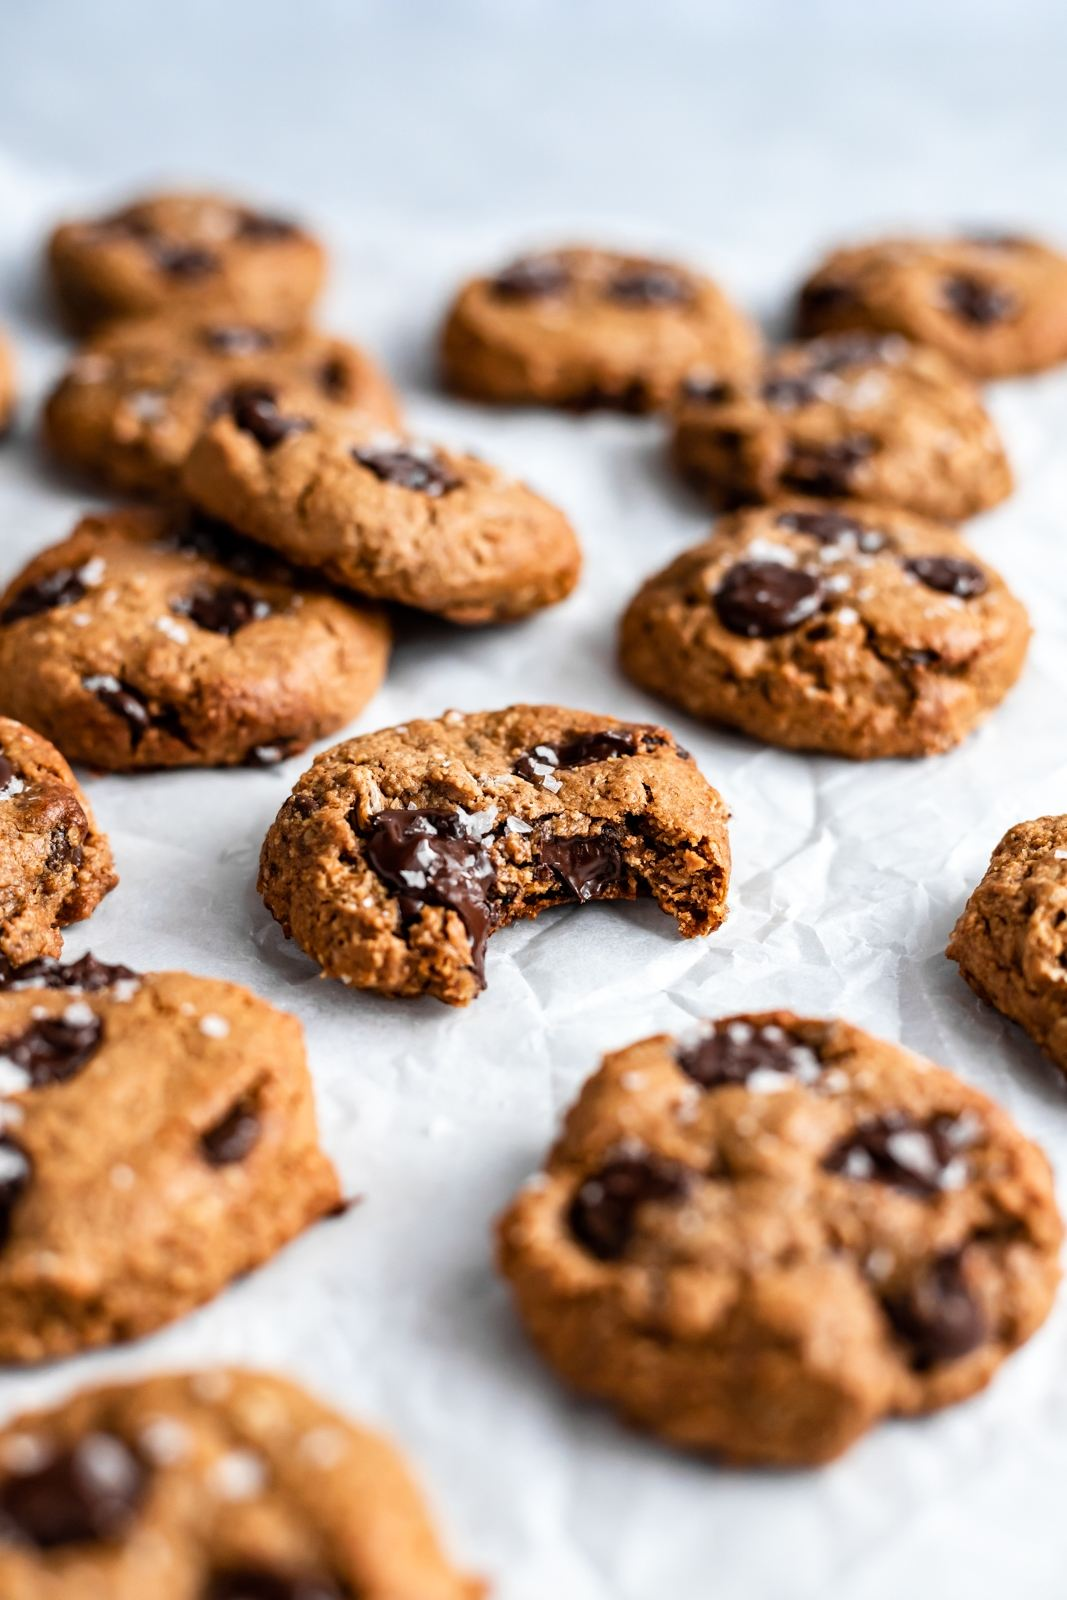
\includegraphics[scale=0.15]{img/C2/2-3/1.png}
\end{figure}

例如用户首次访问Amazon,HTTP响应报文中会包含Set-cookies识别码,浏览器会将识别码添加到所管理的文件中。当用户继续浏览Amazon时,每一个HTTP请求浏览器都会从cookie文件中查询该网站的识别码,并添加到HTTP请求报文中。Amazon也可以通过cookie来维护用户希望购买的商品信息,并推荐个性化产品。

\begin{figure}[H]
    \centering
    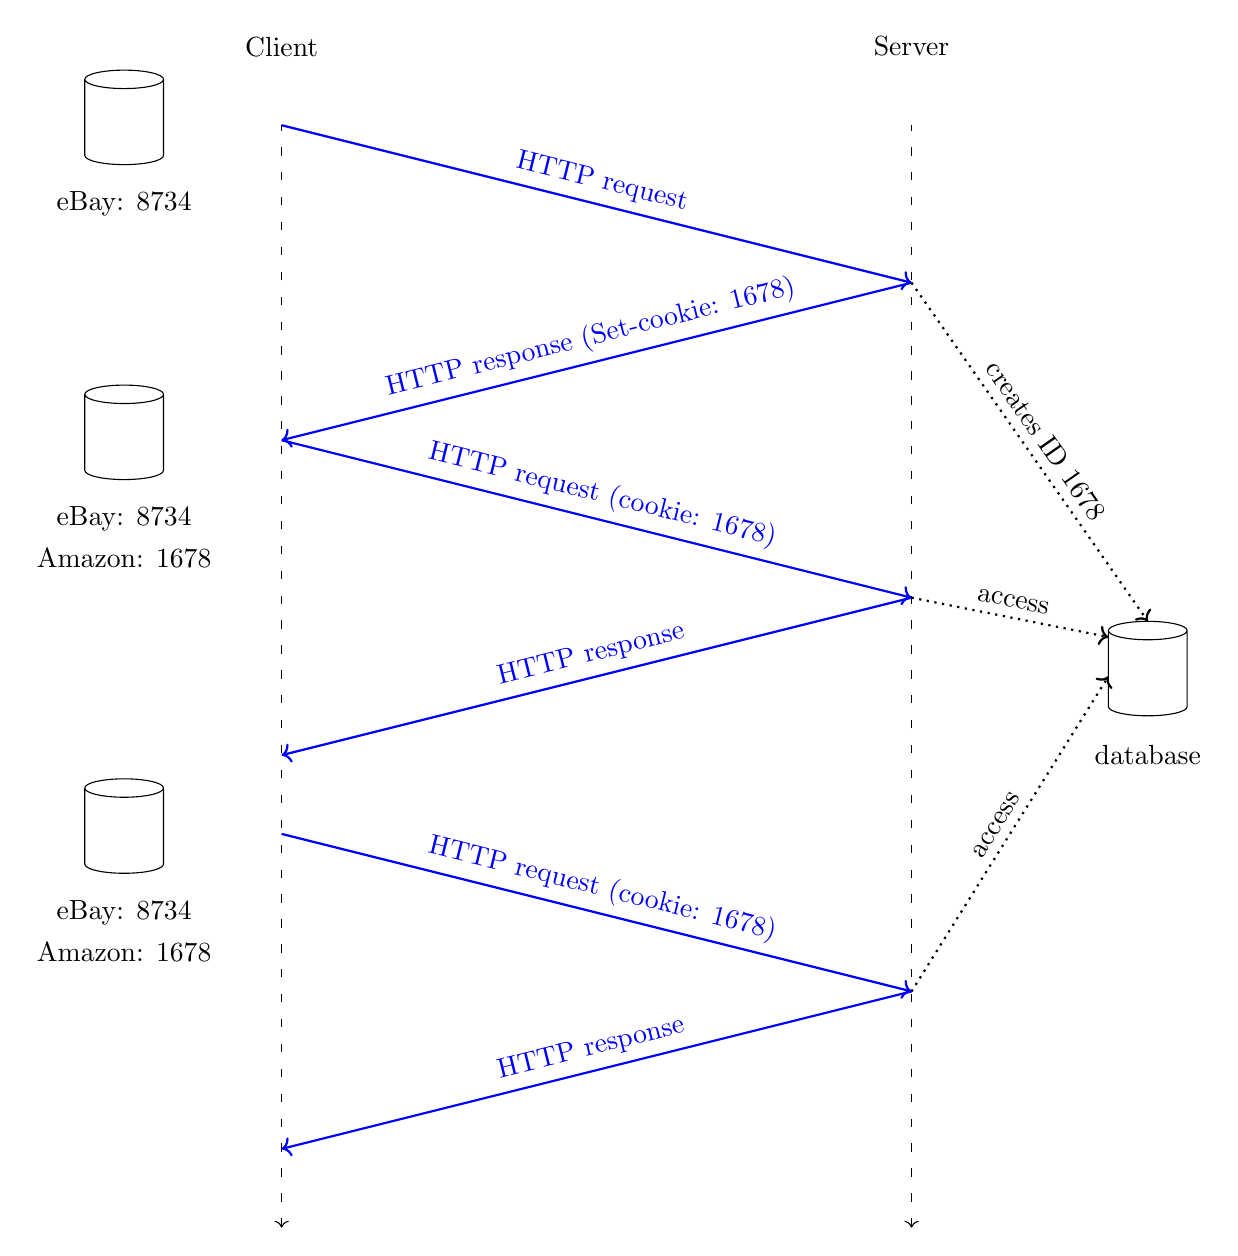
\begin{tikzpicture}
        \node at (0,15) {Client};
        \node at (8,15) {Server};

        \draw[loosely dashed, <-] (0,0) -- (0,14);
        \draw[loosely dashed, <-] (8,0) -- (8,14);

        \draw[blue, ->, thick] (0,14) -- (8,12) node[above, midway, sloped]{HTTP request};
        \draw[blue, ->, thick] (8,12) -- (0,10) node[above, midway, sloped]{HTTP response (Set-cookie: 1678)};
        \draw[blue, ->, thick] (0,10) -- (8,8) node[above, midway, sloped]{HTTP request (cookie: 1678)};
        \draw[blue, ->, thick] (8,8) -- (0,6) node[above, midway, sloped]{HTTP response};
        \draw[blue, ->, thick] (0,5) -- (8,3) node[above, midway, sloped]{HTTP request (cookie: 1678)};
        \draw[blue, ->, thick] (8,3) -- (0,1) node[above, midway, sloped]{HTTP response};

        \node at (-2,14) [cylinder, shape border rotate=90, draw, minimum height=12mm, minimum width=10mm] {};
        \node at (-2,13) {eBay: 8734};

        \node at (-2,10) [cylinder, shape border rotate=90, draw, minimum height=12mm, minimum width=10mm] {};
        \node at (-2,9) {eBay: 8734};
        \node at (-2,8.5) {Amazon: 1678};

        \node at (-2,5) [cylinder, shape border rotate=90, draw, minimum height=12mm, minimum width=10mm] {};
        \node at (-2,4) {eBay: 8734};
        \node at (-2,3.5) {Amazon: 1678};

        \node at (11,7) [cylinder, shape border rotate=90, draw, minimum height=12mm, minimum width=10mm] {};
        \node at (11,6) {database};

        \draw[dotted, ->, thick] (8,12) -- (11,7.7) node[above, midway, sloped]{creates ID 1678};
        \draw[dotted, ->, thick] (8,8) -- (10.5,7.5) node[above, midway, sloped]{access};
        \draw[dotted, ->, thick] (8,3) -- (10.5,7) node[above, midway, sloped]{access};
    \end{tikzpicture}
    \caption{Cookie}
\end{figure}

\newpage

\section{Email}

\subsection{Email}


\chapter{传输层}

\section{多路复用与多路分解}

\subsection{传输层}

传输层协议为运行在不同主机上的应用进程之间提供了逻辑通信。在发送端,运输层将应用进程的报文添加传输层首部形成传输层分组,称为报文段(segment),这个过程被称为多路复用(multiplexing)。在接收端,网络层从数据报中提取传输层报文段,并交付给传输层,传输层处理报文段,将数据交付给应用进程,这个过程被称为多路分解(demultiplexing)。\\

应用层可以使用UDP和TCP这两种截然不同的传输层协议。其中UDP提供了一种不可靠、无连接的服务,因此,UDP不能保证一个进程发送的数据能够完整无缺地到达目的进程。而TCP提供了一种可靠的、面向连接的服务,通过使用流量控制、序号、确认和定时器,TCP确保正确地、按序地将数据交付给接收进程。\\

\subsection{无连接的多路复用/多路分解}

一个UDP的socket是由一个二元组进行标识的,该二元组包含了目的IP地址和目的端口号。如果两个UDP报文段来自不同的源IP地址或源端口号,但是具有相同的目的IP和目的端口号,那么这两个报文段将通过相同的socket被发送到相同的目的进程。\\

使用UDP时,当A给B发送的报文段中,源端口号是用作返回地址的一部分。当B回发一个报文段给A时,就需要从A到B的报文段中取值。\\

\begin{figure}[H]
	\centering
	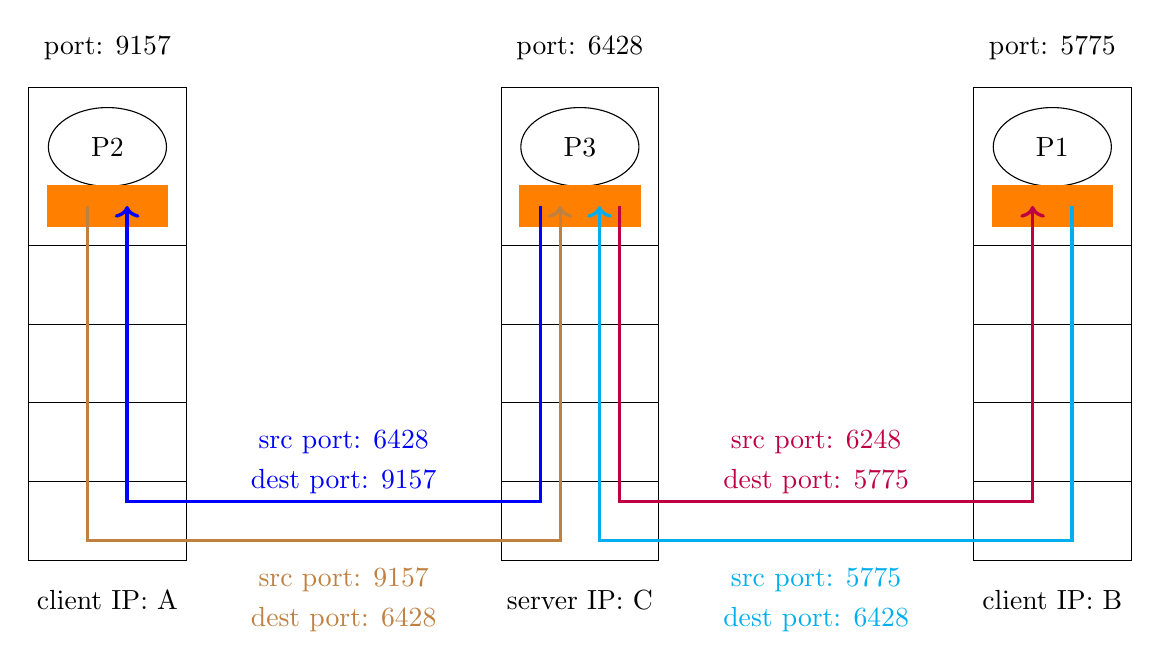
\begin{tikzpicture}
		\draw (1,6.5) node {port: 9157};
		\draw (0,0) rectangle (2,6);
		\draw (0,1) -- (2,1);
		\draw (0,2) -- (2,2);
		\draw (0,3) -- (2,3);
		\draw (0,4) -- (2,4);
		\draw (1,-0.5) node {client IP: A};
		\draw (1,5.25) ellipse (0.75 and 0.5);
		\draw (1,5.25) node {P2};
		\draw[orange, very thick, fill] (0.25,4.25) rectangle (1.75,4.75);

		\draw (7,6.5) node {port: 6428};
		\draw (6,0) rectangle (8,6);
		\draw (6,1) -- (8,1);
		\draw (6,2) -- (8,2);
		\draw (6,3) -- (8,3);
		\draw (6,4) -- (8,4);
		\draw (7,-0.5) node {server IP: C};
		\draw (7,5.25) ellipse (0.75 and 0.5);
		\draw (7,5.25) node {P3};
		\draw[orange, very thick, fill] (6.25,4.25) rectangle (7.75,4.75);

		\draw (13,6.5) node {port: 5775};
		\draw (12,0) rectangle (14,6);
		\draw (12,1) -- (14,1);
		\draw (12,2) -- (14,2);
		\draw (12,3) -- (14,3);
		\draw (12,4) -- (14,4);
		\draw (13,-0.5) node {client IP: B};
		\draw (13,5.25) ellipse (0.75 and 0.5);
		\draw (13,5.25) node {P1};
		\draw[orange, very thick, fill] (12.25,4.25) rectangle (13.75,4.75);

		\draw[->, very thick, brown] (0.75,4.5) -- (0.75,0.25) -- (6.75,0.25) -- (6.75,4.5);
		\draw[brown] (4,-0.25) node {src port: 9157};
		\draw[brown] (4,-0.75) node {dest port: 6428};

		\draw[->, very thick, blue] (6.5,4.5) -- (6.5,0.75) -- (1.25,0.75) -- (1.25,4.5);
		\draw[blue] (4,1.5) node {src port: 6428};
		\draw[blue] (4,1) node {dest port: 9157};

		\draw[->, very thick, cyan] (13.25,4.5) -- (13.25,0.25) -- (7.25,0.25) -- (7.25,4.5);
		\draw[cyan] (10,-0.25) node {src port: 5775};
		\draw[cyan] (10,-0.75) node {dest port: 6428};

		\draw[->, very thick, purple] (7.5,4.5) -- (7.5,0.75) -- (12.75,0.75) -- (12.75,4.5);
		\draw[purple] (10,1.5) node {src port: 6248};
		\draw[purple] (10,1) node {dest port: 5775};
	\end{tikzpicture}
	\caption{无连接的多路复用与多路分解}
\end{figure}

\vspace{0.5cm}

\subsection{面向连接的多路复用与多路分解}

TCP的socket是由一个四元组来标识的,其中包括了源IP地址、源端口号、目的IP地址和目的端口号。与UDP不同的是,两个具有不同源IP地址或源端口号的TCP报文段将被发送到两个不同的socket。\\

\begin{figure}[H]
	\centering
	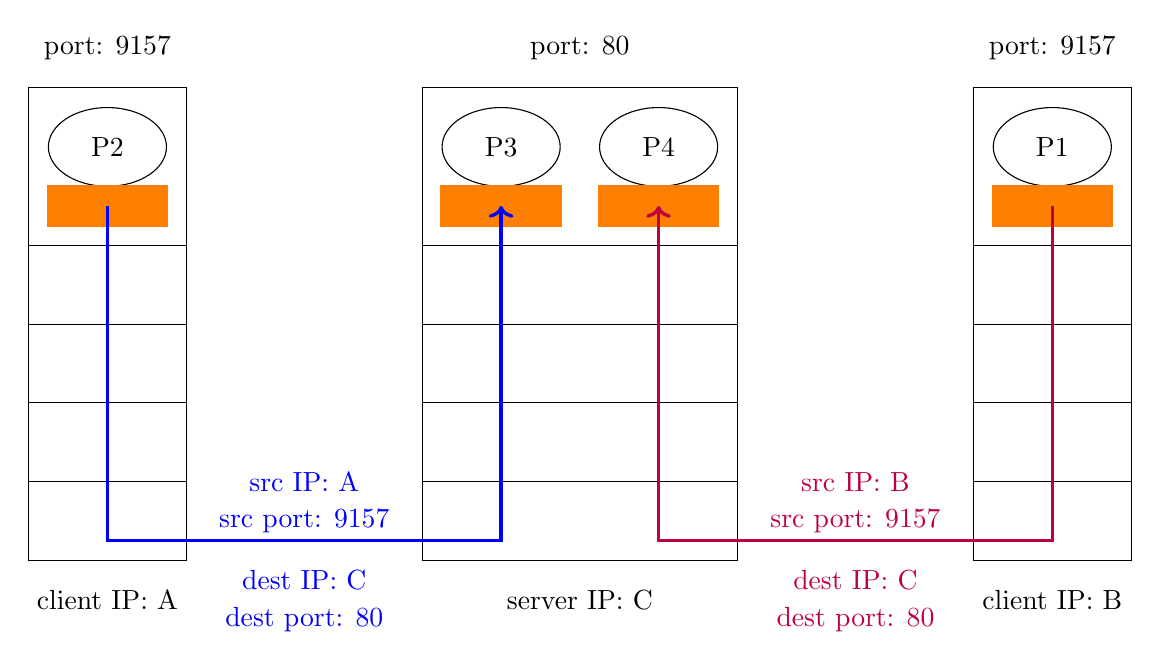
\begin{tikzpicture}
		\draw (1,6.5) node {port: 9157};
		\draw (0,0) rectangle (2,6);
		\draw (0,1) -- (2,1);
		\draw (0,2) -- (2,2);
		\draw (0,3) -- (2,3);
		\draw (0,4) -- (2,4);
		\draw (1,-0.5) node {client IP: A};
		\draw (1,5.25) ellipse (0.75 and 0.5);
		\draw (1,5.25) node {P2};
		\draw[orange, very thick, fill] (0.25,4.25) rectangle (1.75,4.75);

		\draw (7,6.5) node {port: 80};
		\draw (5,0) rectangle (9,6);
		\draw (5,1) -- (9,1);
		\draw (5,2) -- (9,2);
		\draw (5,3) -- (9,3);
		\draw (5,4) -- (9,4);
		\draw (7,-0.5) node {server IP: C};
		\draw (6,5.25) ellipse (0.75 and 0.5);
		\draw (6,5.25) node {P3};
		\draw[orange, very thick, fill] (5.25,4.25) rectangle (6.75,4.75);
		\draw (8,5.25) ellipse (0.75 and 0.5);
		\draw (8,5.25) node {P4};
		\draw[orange, very thick, fill] (7.25,4.25) rectangle (8.75,4.75);

		\draw (13,6.5) node {port: 9157};
		\draw (12,0) rectangle (14,6);
		\draw (12,1) -- (14,1);
		\draw (12,2) -- (14,2);
		\draw (12,3) -- (14,3);
		\draw (12,4) -- (14,4);
		\draw (13,-0.5) node {client IP: B};
		\draw (13,5.25) ellipse (0.75 and 0.5);
		\draw (13,5.25) node {P1};
		\draw[orange, very thick, fill] (12.25,4.25) rectangle (13.75,4.75);

		\draw[->, very thick, blue] (1,4.5) -- (1,0.25) -- (6,0.25) -- (6,4.5);
		\draw[blue] (3.5,1) node {src IP: A};
		\draw[blue] (3.5,0.5) node {src port: 9157};
		\draw[blue] (3.5,-0.25) node {dest IP: C};
		\draw[blue] (3.5,-0.75) node {dest port: 80};

		\draw[->, very thick, purple] (13,4.5) -- (13,0.25) -- (8,0.25) -- (8,4.5);
		\draw[purple] (10.5,1) node {src IP: B};
		\draw[purple] (10.5,0.5) node {src port: 9157};
		\draw[purple] (10.5,-0.25) node {dest IP: C};
		\draw[purple] (10.5,-0.75) node {dest port: 80};
	\end{tikzpicture}
	\caption{面向连接的多路复用与多路分解}
\end{figure}

\newpage

\section{无连接运输UDP}

\subsection{无连接运输UDP}

使用UDP时,在发送报文段之前,发送方和接收方的运输层实体之间没有握手。正因为如此,UDP被称为是无连接的。\\

UDP尽最大努力将数据包交付到目的主机,但不保证可靠性和顺序,也不保证带宽及延迟要求。UDP相较于TCP的优势包括无需连接建立、无连接状态、分组首部开销小。\\

\begin{table}[H]
	\centering
	\begin{tabular}{|p{3cm}<{\centering}|p{3cm}<{\centering}|}
		\hline
		source port \# & dest port \#                    \\
		\hline
		length         & checksum                        \\
		\hline
		\multicolumn{2}{|c|}{application data (message)} \\
		\hline
	\end{tabular}
	\caption{UDP报文段结构}
\end{table}

UDP首部只有4个字段,每个字段由2个字节组成,通过端口号可以将应用数据交给运行在目的端系统中的相应进程。长度字段指示了UDP报文段中的字节数(包括首部)。检验和可以用来检查该报文段中是否出现了差错。\\

\subsection{校验和(Checksum)}

当UDP报文段从源到达目的地的过程中,其中的bit有可能会受到噪声干扰或在路由器中存储而发生改变。UDP检验和提供了差错检测的功能。发送方对UDP报文段中所有内容都当作16位整数进行求和,在求和时遇到的溢出都需要被回卷(wraparound),再对和进行求反,得到的结果被放在UDP报文段中的检验和字段。\\

例如两个16位的整数相加:

\begin{table}[H]
	\centering
	\begin{tabular}{cD{.}{.}{3}}
		  & 1110011001100110  \\
		+ & 1101010101010101  \\
		\hline
		= & 11011101110111011
	\end{tabular}
\end{table}

将溢出位进行回卷:

\begin{table}[H]
	\centering
	\begin{tabular}{cD{.}{.}{3}}
		  & 1011101110111011 \\
		+ & 1                \\
		\hline
		= & 1011101110111100
	\end{tabular}
\end{table}

计算反码得到校验和0100010001000011。\\

接收方收到报文段后,将所有16位整数相加(包括检验和)。如果该分组中没有差错,则计算得到的和将是1111111111111111,否则说明分组中有差错。\\

当检验和错误的时候,该分组一定错误,将会被丢弃。但是当检验和没有错误时,并不能保证分组是完全正确的。虽然UDP提供差错检测,但它对差错恢复无能无力。

\newpage

\section{可靠数据传输}

\subsection{可靠数据传输(RDT, Reliable Data Transfer)}

由于可靠数据传输协议的下层协议也许是不可靠的,信道的不可靠特性决定了可靠数据传输协议的复杂性,例如TCP就是在不可靠的端到端网络层之上实现的可靠数据传输协议。\\

\begin{figure}[H]
	\centering
	\begin{tikzpicture}
		\draw (0,10) node {应用层};
		\draw (0,5) node {传输层};
		\draw (0,0) node {网络层};
		\draw[dashed] (0,7.5) -- (14,7.5);
		\draw[dashed] (0,2.5) -- (14,2.5);

		\draw (2,12) rectangle (3,13);
		\draw (5,12) rectangle (6,13);
		\draw (8,12) rectangle (9,13);
		\draw (11,12) rectangle (12,13);

		\draw (2.5,10) ellipse (0.75 and 0.5);
		\draw (2.5,10) node {发送};
		\draw (5.5,10) ellipse (0.75 and 0.5);
		\draw (5.5,10) node {接收};

		\node at (4.3,5) [cylinder, shape border rotate=180, draw, minimum height=2.5cm, minimum width=1cm]{可靠信道};
		\draw[->, very thick] (2.5,9.5) -- (2.5,5) -- (3,5);
		\draw[->, very thick] (5.4,5) -- (5.5,5) -- (5.5,9.5);

		\node at (10.3,0) [cylinder, shape border rotate=180, draw, minimum height=2.5cm, minimum width=1cm]{不可靠信道};
		\draw (7.5,4.5) rectangle (9.5,5.5);
		\draw (8.5,5) node {rdt};
		\draw (10.5,4.5) rectangle (12.5,5.5);
		\draw (11.5,5) node {rdt};

		\draw[->, very thick] (8.5,9) -- (8.5,5.5);
		\draw[->, very thick] (8.5,4.5) -- (8.5,0) -- (8.8,0);
		\draw[->, very thick] (11.5,0) -- (11.5,4.5);
		\draw[->, very thick] (11.5,5.5) -- (11.5,9);

		\draw (7,6.5) node {rdt\_send()};
		\draw (7,3.5) node {udt\_send()};
		\draw (13,6.5) node {deliver\_data()};
		\draw (13,3.5) node {udt\_rcv()};
	\end{tikzpicture}
	\caption{可靠数据传输}
\end{figure}

\vspace{0.5cm}

\subsection{rdt 1.0:经完全可靠信道的可靠数据传输}

考虑最简单的情况,假设底层信道是完全可靠的(不会出错、不会丢失)。有限状态机(FSM, Finite State Machine)可以用于描述发送方和接收方的操作。\\

\begin{figure}[H]
	\centering
	\begin{tikzpicture}
		\node[state, initial, draw, align=center] (s1) {wait for\\call};
		\draw (s1) edge[loop right] node{} (s1);
		\draw (5,0.5) node {rdt\_send(data)};
		\draw (2.5,0.25) -- (7.5,0.25);
		\draw (5,0) node {pkt = make\_pkt(data)};
		\draw (4.25,-0.5) node {udt\_send(pkt)};
	\end{tikzpicture}
	\caption{rdt 1.0发送端}
\end{figure}

\vspace{0.5cm}

\begin{figure}[H]
	\centering
	\begin{tikzpicture}
		\node[state, initial, draw, align=center] (s1) {wait for\\call};
		\draw (s1) edge[loop right] node{} (s1);
		\draw (5.5,0.5) node {rdt\_rcv(pkt)};
		\draw (3,0.25) -- (8,0.25);
		\draw (5.3,0) node {data = extract(pkt)};
		\draw (5.2,-0.5) node {deliver\_data(data)};
	\end{tikzpicture}
	\caption{rdt 1.0接收端}
\end{figure}

\vspace{0.5cm}

\subsection{rdt 2.0:经具有比特差错信道的可靠数据传输}

在分组的传输、传播或缓存的过程中,分组中的比特可能会受损。类似于打电话,当接听电话的人听到并理解一句话时会说“OK”,但如果没听清,就会要求对方再说一遍。\\

rdt 2.0增加了差错检验、接收方反馈和重传机制。当接收方接收到正确的报文时,就给对方一个肯定确认(ACK, positive acknowledgment),告诉他“没问题”。当接收方检测到报文错误时,就需要给对方一个否定确认(NAK, negative acknowledgment),告诉对方“你给我发的不对,重新给我发一份新的吧”。\\

\begin{figure}[H]
	\centering
	\begin{tikzpicture}[node distance=5cm]
		\node[state, initial, draw, align=center] (s1) {wait for\\call};
		\node[state, right of=s1, draw, align=center] (s2) {wait for\\ACK/NAK};

		\draw[->] (s1) edge[above, bend left] node{} (s2);
		\draw[->] (s2) edge[above, bend left] node{} (s1);
		\draw[->] (s2) edge[loop right] node{} (s2);

		\draw (0,3) node {rdt\_send(data)};
		\draw (-2.5,2.75) -- (2.5,2.75);
		\draw (0,2.5) node {sndpkt = make\_pkt(data)};
		\draw (-0.8,2) node {udt\_send(sndpkt)};

		\draw (9,2) node {rdt\_rcv(rcvpkt) \&\& is\_nak(rcvpkt)};
		\draw (5.5,1.75) -- (12.5,1.75);
		\draw (9,1.5) node {udt\_send(sndpkt)};

		\draw (3,-2) node {rdt\_rcv(rcvpkt) \&\& is\_ack(rcvpkt)};
		\draw (-0.5,-2.25) -- (6.5,-2.25);
		\draw (3,-2.5) node {$ \wedge $};
	\end{tikzpicture}
	\caption{rdt 2.0发送端}
\end{figure}

\vspace{0.5cm}

\begin{figure}[H]
	\centering
	\begin{tikzpicture}
		\node[state, initial, draw, align=center] (s1) {wait for\\call};
		\draw (s1) edge[loop above] node{} (s1);
		\draw (s1) edge[loop below] node{} (s1);

		\draw (4,3) node {rdt\_rcv(rcvpkt) \&\& corrupt(rcvpkt)};
		\draw (0.5,2.75) -- (7.5,2.75);
		\draw (3.5,2.5) node {sndpkt = make\_pkt(NAK)};
		\draw (2.65,2) node {udt\_send(sndpkt)};

		\draw (4,-1.5) node {rdt\_rcv(rcvpkt) \&\& !corrupt(rcvpkt)};
		\draw (0.5,-1.75) -- (7.5,-1.75);
		\draw (3.5,-2) node {data = extract(rcvpkt)};
		\draw (3.15,-2.5) node {deliver\_data(data)};
		\draw (3.95,-3) node {sndpkt = make\_pkt(ACK)};
		\draw (3.1,-3.5) node {udt\_send(sndpkt)};
	\end{tikzpicture}
	\caption{rdt 2.0接收端}
\end{figure}

\vspace{0.5cm}

发送方在将分组发送后,等待来自接收方的ACK或NAK。如果收到ACK,则代表接收方正确地接收了分组,那么就回到初始状态继续等待上层的数据。如果收到NAK,那就表示接收方没有收到正确的分组,需要进行重传并且继续处于等待ACK或NAK的状态。像这种只有当发送方接收到ACK后才能够继续发送新的报文的协议,被称为停等协议(stop-and-wait)。\\

rdt 2.0看起来似乎可以运行了,但遗憾的是,它存在一个致命的缺陷——ACK或NAK也存在受损的可能性!\\

当发送方收到的是一个受损的ACK或NAK时,如果发送方简单地选择直接重发分组会导致接收方收到重复的分组。\\

\subsection{rdt 2.1:带序号消息协议}

发送方可以为分组添加序号,接收方只需检查需要就可确定收到的分组是否重复。对于停等协议而言,序号只需要使用0和1就可以了。\\

\begin{figure}[H]
	\centering
	\begin{tikzpicture}[node distance=5cm]
		\node[state, initial, draw, align=center] (s1) {wait for\\call 0};
		\node[state, right of=s1, draw, align=center] (s2) {wait for\\ACK/NAK 0};
		\node[state, below of=s2, draw, align=center] (s3) {wait for\\call 1};
		\node[state, left of=s3, draw, align=center] (s4) {wait for\\ACK/NAK 1};

		\draw[->] (s1) edge[above, bend left] node{} (s2);
		\draw[->] (s2) edge[loop right] node{} (s2);
		\draw[->] (s2) edge[above, bend left] node{} (s3);
		\draw[->] (s3) edge[above, bend left] node{} (s4);
		\draw[->] (s4) edge[loop left] node{} (s4);
		\draw[->] (s4) edge[above, bend left] node{} (s1);

		\draw (3,3) node {rdt\_send(data)};
		\draw (0,2.75) -- (6,2.75);
		\draw (3,2.5) node {sndpkt = make\_pkt(0, data)};
		\draw (2,2) node {udt\_send(sndpkt)};

		\draw (8.5,2.5) node {rdt\_rcv(rcvpkt) \&\&};
		\draw (8.3,2) node {(corrupt(rcvpkt) ||};
		\draw (8.1,1.5) node {is\_nak(rcvpkt))};
		\draw (6.5,1.25) -- (10.5,1.25);
		\draw (8.5,1) node {udt\_send(sndpkt)};

		\draw (8,-2) node {rdt\_rcv(rcvpkt) \&\&};
		\draw (8,-2.5) node {!corrupt(rcvpkt) \&\&};
		\draw (7.6,-3) node {is\_ack(rcvpkt))};
		\draw (6,-3.25) -- (10,-3.25);
		\draw (7.5,-3.5) node {$ \wedge $};

		\draw (4,-7) node {rdt\_send(data)};
		\draw (1,-7.25) -- (7,-7.25);
		\draw (4,-7.5) node {sndpkt = make\_pkt(1, data)};
		\draw (3,-8) node {udt\_send(sndpkt)};

		\draw (-2,-7) node {rdt\_rcv(rcvpkt) \&\&};
		\draw (-2.2,-7.5) node {(corrupt(rcvpkt) ||};
		\draw (-2.4,-8) node {is\_nak(rcvpkt))};
		\draw (-4,-8.25) -- (0,-8.25);
		\draw (-2,-8.5) node {udt\_send(sndpkt)};

		\draw (-3,-2) node {rdt\_rcv(rcvpkt) \&\&};
		\draw (-3,-2.5) node {!corrupt(rcvpkt) \&\&};
		\draw (-3.4,-3) node {is\_ack(rcvpkt))};
		\draw (-5,-3.25) -- (-1,-3.25);
		\draw (-3,-3.5) node {$ \wedge $};
	\end{tikzpicture}
	\caption{rdt 2.1发送端}
\end{figure}

\vspace{0.5cm}

\begin{figure}[H]
	\centering
	\begin{tikzpicture}[node distance=5cm]
		\node[state, initial, draw, align=center] (s1) {wait for\\call 0};
		\node[state, right of=s1, draw, align=center] (s2) {wait for\\call 1};

		\draw[->] (s1) edge[above, bend left] node{} (s2);
		\draw[->] (s2) edge[above, bend left] node{} (s1);
		\draw[->] (s1) edge[loop above] node{} (s1);
		\draw[->] (s1) edge[loop below] node{} (s1);
		\draw[->] (s2) edge[loop above] node{} (s2);
		\draw[->] (s2) edge[loop below] node{} (s2);

		\draw (2.5,5) node {rdt\_rcv(rcvpkt) \&\&};
		\draw (2.5,4.5) node {!corrupt(rcvpkt) \&\&};
		\draw (2.2,4) node {has\_seq0(rcvpkt)};
		\draw (0.3,3.75) -- (5.7,3.75);
		\draw (2.6,3.5) node {data = extract(rcvpkt)};
		\draw (2.25,3) node {deliver\_data(data)};
		\draw (3,2.5) node {sndpkt = make\_pkt(ACK)};
		\draw (2.2,2) node {udt\_send(sndpkt)};

		\draw (-3.4,3) node {rdt\_rcv(rcvpkt) \&\&};
		\draw (-3.85,2.5) node {corrupt(rcvpkt)};
		\draw (-5.5,2.25) -- (-0.3,2.25);
		\draw (-2.75,2) node {sndpkt = make\_pkt(NAK)};
		\draw (-3.6,1.5) node {udt\_send(sndpkt)};

		\draw (-3.5,-2) node {rdt\_rcv(rcvpkt) \&\&};
		\draw (-3.5,-2.5) node {!corrupt(rcvpkt) \&\&};
		\draw (-3.7,-3) node {has\_seq1(rcvpkt)};
		\draw (-5.5,-3.25) -- (-0.3,-3.25);
		\draw (-2.8,-3.5) node {sndpkt = make\_pkt(ACK)};
		\draw (-3.65,-4) node {udt\_send(sndpkt)};

		\draw (2.5,-2) node {rdt\_rcv(rcvpkt) \&\&};
		\draw (2.5,-2.5) node {!corrupt(rcvpkt) \&\&};
		\draw (2.2,-3) node {has\_seq1(rcvpkt)};
		\draw (0.3,-3.25) -- (5.7,-3.25);
		\draw (2.6,-3.5) node {data = extract(rcvpkt)};
		\draw (2.25,-4) node {deliver\_data(data)};
		\draw (3,-4.5) node {sndpkt = make\_pkt(ACK)};
		\draw (2.2,-5) node {udt\_send(sndpkt)};

		\draw (7.7,3) node {rdt\_rcv(rcvpkt) \&\&};
		\draw (7.2,2.5) node {corrupt(rcvpkt)};
		\draw (5.5,2.25) -- (11,2.25);
		\draw (8.3,2) node {sndpkt = make\_pkt(NAK)};
		\draw (7.45,1.5) node {udt\_send(sndpkt)};

		\draw (8,-2) node {rdt\_rcv(rcvpkt) \&\&};
		\draw (8,-2.5) node {!corrupt(rcvpkt) \&\&};
		\draw (7.75,-3) node {has\_seq0(rcvpkt)};
		\draw (6,-3.25) -- (11.25,-3.25);
		\draw (8.65,-3.5) node {sndpkt = make\_pkt(ACK)};
		\draw (7.8,-4) node {udt\_send(sndpkt)};
	\end{tikzpicture}
	\caption{rdt 2.1接收端}
\end{figure}

\vspace{0.5cm}

\subsection{rdt 2.2:无NAK消息协议}

rdt 2.2与同rdt 2.1的功能相同,但是只使用ACK。接收方每次ACK最后一个被正确接收的分组,当发送方收到重复的ACK之后,采用与NAK相同的处理动作,将分组重传给接收方。\\

\begin{figure}[H]
	\centering
	\begin{tikzpicture}[node distance=4cm]
		\node[state, initial, draw, align=center] (s1) {wait for\\call 0};
		\node[state, right of=s1, draw, align=center] (s2) {wait for\\ACK 0};
		\node[state, below of=s2, draw, align=center] (s3) {wait for\\call 1};
		\node[state, left of=s3, draw, align=center] (s4) {wait for\\ACK 1};

		\draw[->] (s1) edge[above, bend left] node{} (s2);
		\draw[->] (s2) edge[loop right] node{} (s2);
		\draw[->] (s2) edge[above, bend left] node{} (s3);
		\draw[->] (s3) edge[above, bend left] node{} (s4);
		\draw[->] (s4) edge[loop left] node{} (s4);
		\draw[->] (s4) edge[above, bend left] node{} (s1);

		\draw (3,3) node {rdt\_send(data)};
		\draw (0,2.75) -- (6,2.75);
		\draw (3,2.5) node {sndpkt = make\_pkt(0, data)};
		\draw (2,2) node {udt\_send(sndpkt)};

		\draw (8.5,2.5) node {rdt\_rcv(rcvpkt) \&\&};
		\draw (8.3,2) node {(corrupt(rcvpkt) ||};
		\draw (8.3,1.5) node {is\_ack(rcvpkt, 1))};
		\draw (6.5,1.25) -- (10.5,1.25);
		\draw (8.5,1) node {udt\_send(sndpkt)};

		\draw (8,-1.5) node {rdt\_rcv(rcvpkt) \&\&};
		\draw (8,-2) node {!corrupt(rcvpkt) \&\&};
		\draw (7.9,-2.5) node {is\_ack(rcvpkt, 0))};
		\draw (6,-2.75) -- (10,-2.75);
		\draw (7.5,-3) node {$ \wedge $};

		\draw (4,-6) node {rdt\_send(data)};
		\draw (1,-6.25) -- (7,-6.25);
		\draw (4,-6.5) node {sndpkt = make\_pkt(1, data)};
		\draw (3,-7) node {udt\_send(sndpkt)};

		\draw (-2,-5.5) node {rdt\_rcv(rcvpkt) \&\&};
		\draw (-2.2,-6) node {(corrupt(rcvpkt) ||};
		\draw (-2.2,-6.5) node {is\_ack(rcvpkt, 0))};
		\draw (-4,-6.75) -- (0,-6.75);
		\draw (-2,-7) node {udt\_send(sndpkt)};

		\draw (-3,-1.5) node {rdt\_rcv(rcvpkt) \&\&};
		\draw (-3,-2) node {!corrupt(rcvpkt) \&\&};
		\draw (-3.2,-2.5) node {is\_ack(rcvpkt, 1))};
		\draw (-5,-2.75) -- (-1,-2.75);
		\draw (-3,-3) node {$ \wedge $};
	\end{tikzpicture}
	\caption{rdt 2.2发送端}
\end{figure}

\vspace{0.5cm}

\begin{figure}[H]
	\centering
	\begin{tikzpicture}[node distance=5cm]
		\draw[->] (-1,2) -- (-0.6,0.9);
		\draw (-1.5,1.5) node {start};

		\node[state, draw, align=center] (s1) {wait for\\call 0};
		\node[state, right of=s1, draw, align=center] (s2) {wait for\\call 1};

		\draw[->] (s1) edge[above, bend left] node{} (s2);
		\draw[->] (s2) edge[above, bend left] node{} (s1);
		\draw[->] (s1) edge[loop left] node{} (s1);
		\draw[->] (s2) edge[loop right] node{} (s2);

		\draw (1.8,5) node {rdt\_rcv(rcvpkt) \&\&};
		\draw (1.8,4.5) node {!corrupt(rcvpkt) \&\&};
		\draw (1.5,4) node {has\_seq0(rcvpkt)};
		\draw (-0.4,3.75) -- (5.5,3.75);
		\draw (1.9,3.5) node {data = extract(rcvpkt)};
		\draw (1.55,3) node {deliver\_data(data)};
		\draw (2.55,2.5) node {sndpkt = make\_pkt(ACK, 0)};
		\draw (1.5,2) node {udt\_send(sndpkt)};

		\draw (-3.5,-1) node {rdt\_rcv(rcvpkt) \&\&};
		\draw (-3.5,-1.5) node {(corrupt(rcvpkt) \&\&};
		\draw (-3.7,-2) node {has\_seq1(rcvpkt))};
		\draw (-5.5,-2.25) -- (0.5,-2.25);
		\draw (-2.65,-2.5) node {sndpkt = make\_pkt(ACK, 1)};
		\draw (-3.7,-3) node {udt\_send(sndpkt)};

		\draw (2.7,-1.5) node {rdt\_rcv(rcvpkt) \&\&};
		\draw (2.7,-2) node {!corrupt(rcvpkt) \&\&};
		\draw (2.4,-2.5) node {has\_seq1(rcvpkt)};
		\draw (0.5,-2.75) -- (5.9,-2.75);
		\draw (2.8,-3) node {data = extract(rcvpkt)};
		\draw (2.45,-3.5) node {deliver\_data(data)};
		\draw (3.4,-4) node {sndpkt = make\_pkt(ACK, 1)};
		\draw (2.4,-4.5) node {udt\_send(sndpkt)};

		\draw (7.7,3.5) node {rdt\_rcv(rcvpkt) \&\&};
		\draw (7.5,3) node {(corrupt(rcvpkt) ||};
		\draw (7.5,2.5) node {has\_seq0(rcvpkt))};
		\draw (5.5,2.25) -- (11.5,2.25);
		\draw (8.5,2) node {sndpkt = make\_pkt(ACK, 0)};
		\draw (7.45,1.5) node {udt\_send(sndpkt)};
	\end{tikzpicture}
	\caption{rdt 2.2接收端}
\end{figure}

\vspace{0.5cm}

\subsection{rdt 3.0:经具有比特差错的丢包信道的可靠数据传输}

假设现在信道既可能发生错误,也可能会丢失分组。如果发送端发送的数据在半路就丢失了,那么发送方就会无休止的等待,接收方没有收到数据,也会处于等待的状态。\\

因此发送方需要一个倒计时定时器(countdown timer),如果发送方在规定时间内没有收到ACK,就将该分组重传。另一种情况是,如果发送的分组并没有丢失,只是延误到达了,这样也会触发定时器重发。但是接收方可以根据分组的序号丢弃重复的分组。\\

\begin{figure}[H]
	\centering
	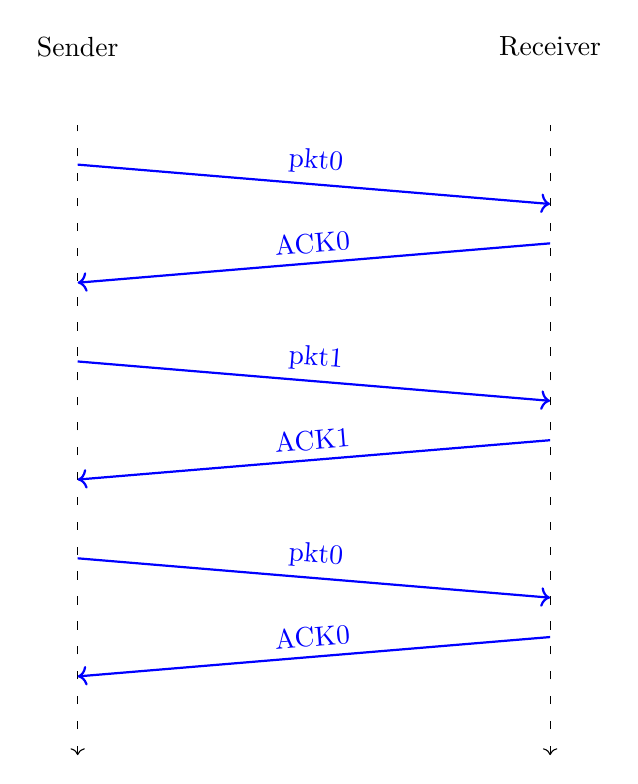
\begin{tikzpicture}
		\node at (0,9) {Sender};
		\node at (6,9) {Receiver};

		\draw[loosely dashed, <-] (0,0) -- (0,8);
		\draw[loosely dashed, <-] (6,0) -- (6,8);

		\draw[blue, ->, thick] (0,7.5) -- (6,7) node[above, midway, sloped]{pkt0};
		\draw[blue, ->, thick] (6,6.5) -- (0,6) node[above, midway, sloped]{ACK0};
		\draw[blue, ->, thick] (0,5) -- (6,4.5) node[above, midway, sloped]{pkt1};
		\draw[blue, ->, thick] (6,4) -- (0,3.5) node[above, midway, sloped]{ACK1};
		\draw[blue, ->, thick] (0,2.5) -- (6,2) node[above, midway, sloped]{pkt0};
		\draw[blue, ->, thick] (6,1.5) -- (0,1) node[above, midway, sloped]{ACK0};
	\end{tikzpicture}
	\caption{无丢包}
\end{figure}

\vspace{0.5cm}

\begin{figure}[H]
	\centering
	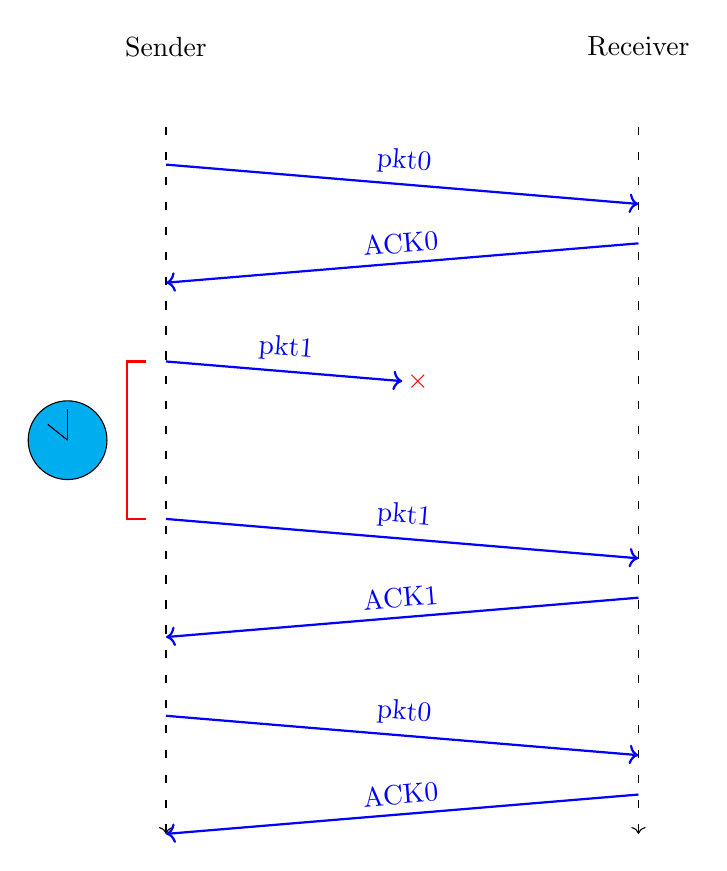
\begin{tikzpicture}
		\node at (0,10) {Sender};
		\node at (6,10) {Receiver};

		\draw[loosely dashed, <-] (0,0) -- (0,9);
		\draw[loosely dashed, <-] (6,0) -- (6,9);

		\draw[blue, ->, thick] (0,8.5) -- (6,8) node[above, midway, sloped]{pkt0};
		\draw[blue, ->, thick] (6,7.5) -- (0,7) node[above, midway, sloped]{ACK0};
		\draw[blue, ->, thick] (0,6) -- (3,5.75) node[above, midway, sloped]{pkt1};
		\node[very thick, red] at (3.2,5.75) {$ \times $};
		\draw[blue, ->, thick] (0,4) -- (6,3.5) node[above, midway, sloped]{pkt1};
		\draw[blue, ->, thick] (6,3) -- (0,2.5) node[above, midway, sloped]{ACK1};
		\draw[blue, ->, thick] (0,1.5) -- (6,1) node[above, midway, sloped]{pkt0};
		\draw[blue, ->, thick] (6,0.5) -- (0,0) node[above, midway, sloped]{ACK0};

		\draw[red, thick] (-0.25,6) -- (-0.5,6) -- (-0.5,4) -- (-0.25,4);
		\filldraw [fill=cyan] (-1.25,5) circle [radius=0.5cm];
		\draw (-1.25,5) -- (-1.25,5.4);
		\draw (-1.25,5) -- (-1.5,5.2);
	\end{tikzpicture}
	\caption{分组丢失}
\end{figure}

\vspace{0.5cm}

\begin{figure}[H]
	\centering
	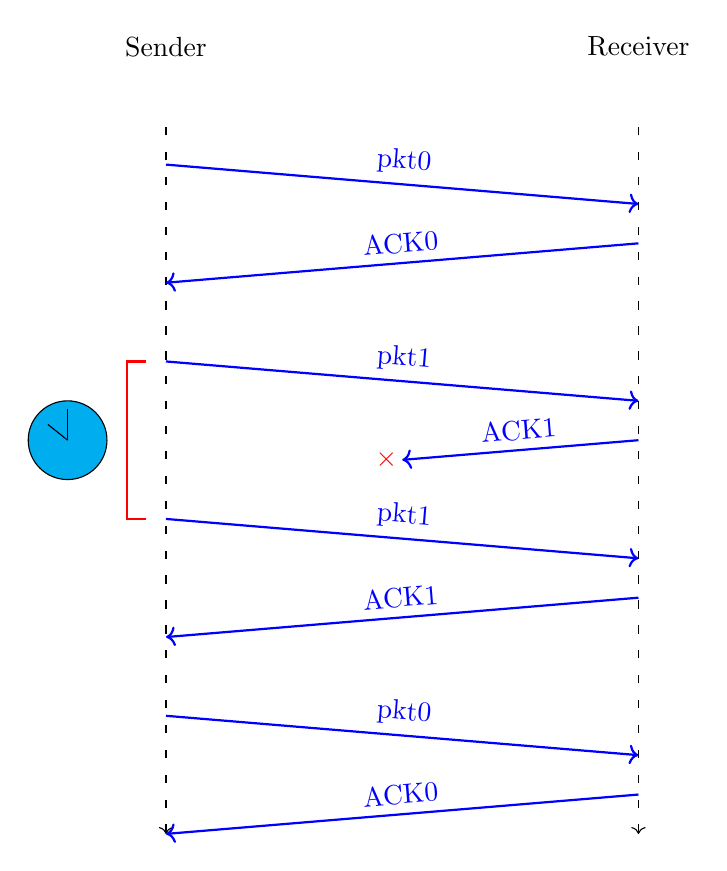
\begin{tikzpicture}
		\node at (0,10) {Sender};
		\node at (6,10) {Receiver};

		\draw[loosely dashed, <-] (0,0) -- (0,9);
		\draw[loosely dashed, <-] (6,0) -- (6,9);

		\draw[blue, ->, thick] (0,8.5) -- (6,8) node[above, midway, sloped]{pkt0};
		\draw[blue, ->, thick] (6,7.5) -- (0,7) node[above, midway, sloped]{ACK0};
		\draw[blue, ->, thick] (0,6) -- (6,5.5) node[above, midway, sloped]{pkt1};
		\draw[blue, ->, thick] (6,5) -- (3,4.75) node[above, midway, sloped]{ACK1};
		\node[very thick, red] at (2.8,4.75) {$ \times $};
		\draw[blue, ->, thick] (0,4) -- (6,3.5) node[above, midway, sloped]{pkt1};
		\draw[blue, ->, thick] (6,3) -- (0,2.5) node[above, midway, sloped]{ACK1};
		\draw[blue, ->, thick] (0,1.5) -- (6,1) node[above, midway, sloped]{pkt0};
		\draw[blue, ->, thick] (6,0.5) -- (0,0) node[above, midway, sloped]{ACK0};

		\draw[red, thick] (-0.25,6) -- (-0.5,6) -- (-0.5,4) -- (-0.25,4);
		\filldraw [fill=cyan] (-1.25,5) circle [radius=0.5cm];
		\draw (-1.25,5) -- (-1.25,5.4);
		\draw (-1.25,5) -- (-1.5,5.2);
	\end{tikzpicture}
	\caption{ACK丢失}
\end{figure}

\vspace{0.5cm}

\begin{figure}[H]
	\centering
	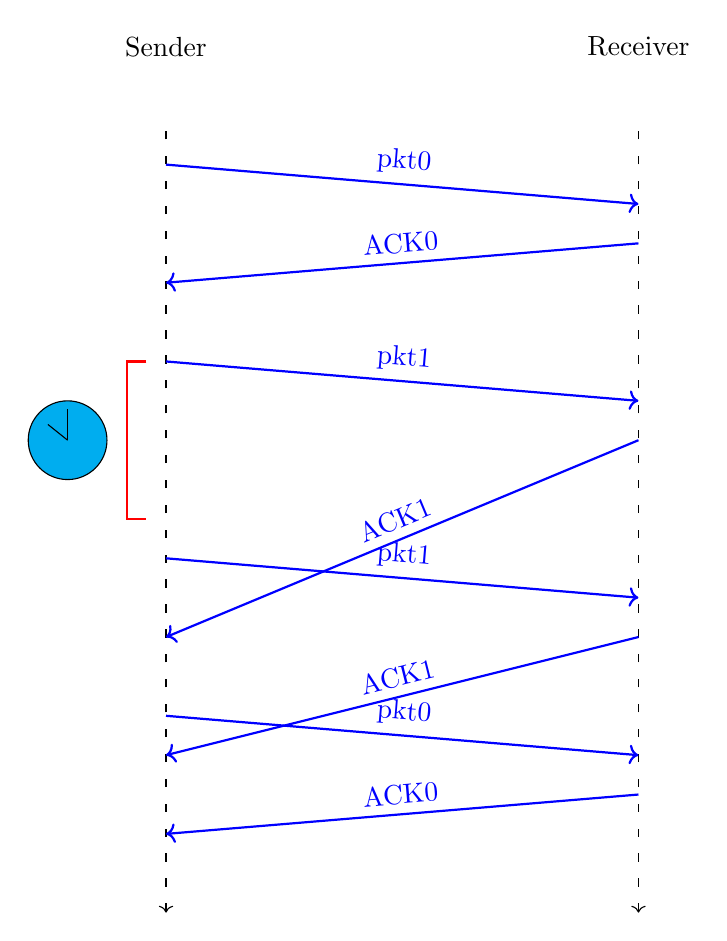
\begin{tikzpicture}
		\node at (0,11) {Sender};
		\node at (6,11) {Receiver};

		\draw[loosely dashed, <-] (0,0) -- (0,10);
		\draw[loosely dashed, <-] (6,0) -- (6,10);

		\draw[blue, ->, thick] (0,9.5) -- (6,9) node[above, midway, sloped]{pkt0};
		\draw[blue, ->, thick] (6,8.5) -- (0,8) node[above, midway, sloped]{ACK0};
		\draw[blue, ->, thick] (0,7) -- (6,6.5) node[above, midway, sloped]{pkt1};
		\draw[blue, ->, thick] (6,6) -- (0,3.5) node[above, midway, sloped]{ACK1};
		\draw[blue, ->, thick] (0,4.5) -- (6,4) node[above, midway, sloped]{pkt1};
		\draw[blue, ->, thick] (6,3.5) -- (0,2) node[above, midway, sloped]{ACK1};
		\draw[blue, ->, thick] (0,2.5) -- (6,2) node[above, midway, sloped]{pkt0};
		\draw[blue, ->, thick] (6,1.5) -- (0,1) node[above, midway, sloped]{ACK0};

		\draw[red, thick] (-0.25,7) -- (-0.5,7) -- (-0.5,5) -- (-0.25,5);
		\filldraw [fill=cyan] (-1.25,6) circle [radius=0.5cm];
		\draw (-1.25,6) -- (-1.25,6.4);
		\draw (-1.25,6) -- (-1.5,6.2);
	\end{tikzpicture}
	\caption{过早超时}
\end{figure}

\vspace{0.5cm}

rdt 3.0能够正确工作,但是性能很差。因为停等协议,导致了发送方的利用率很低。

\newpage

\section{流水线}

\subsection{流水线(Pipelining)}

为了提高发送方的利用率,可以不以停等方式运行,而是采用流水线协议,允许发送方在收到ACK之前连续发送多个分组。\\

使用流水线协议,就需要更大的序列号范围,因为每个输送中的分组必须有一个唯一的序号。同时发送方和接收方需要更大的存储空间以缓存分组。\\

\begin{figure}[H]
	\centering
	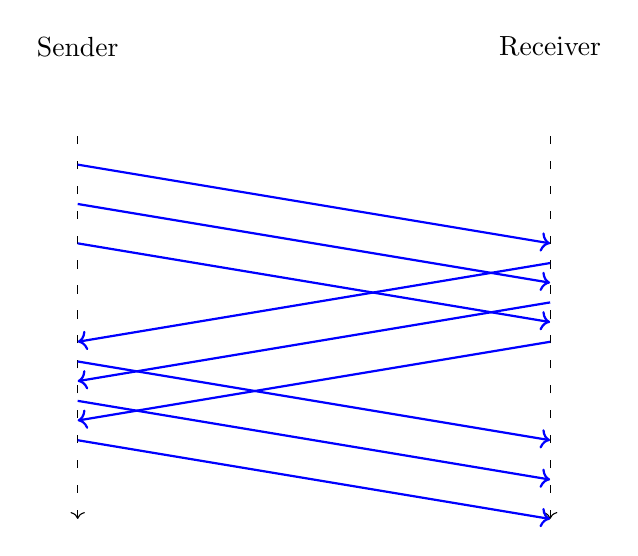
\begin{tikzpicture}
		\node at (0,6) {Sender};
		\node at (6,6) {Receiver};

		\draw[loosely dashed, <-] (0,0) -- (0,5);
		\draw[loosely dashed, <-] (6,0) -- (6,5);

		\draw[blue, ->, thick] (0,4.5) -- (6,3.5);
		\draw[blue, ->, thick] (0,4) -- (6,3);
		\draw[blue, ->, thick] (0,3.5) -- (6,2.5);
		\draw[blue, ->, thick] (6,3.25) -- (0,2.25);
		\draw[blue, ->, thick] (6,2.75) -- (0,1.75);
		\draw[blue, ->, thick] (6,2.25) -- (0,1.25);
		\draw[blue, ->, thick] (0,2) -- (6,1);
		\draw[blue, ->, thick] (0,1.5) -- (6,0.5);
		\draw[blue, ->, thick] (0,1) -- (6,0);
	\end{tikzpicture}
	\caption{流水线}
\end{figure}

解决流水线的差错恢复有两种基本方法:

\begin{enumerate}
    \item Go Back N

    \item 选择重传(Selective Repeat)
\end{enumerate}



\end{document}